% main.tex -- Admissibility Certification for Financial Regime Detectors
% v5 editorial transformation, 2026-07-10.
% Lineage: seeded from the VolRegime-Engine evidence package (2026-06-25);
% the protocol was implemented in the repository under the working name GCDE
% (gauge-calibrated detector exclusion); artifact key names retain that legacy
% vocabulary. See the Reproducibility appendix for the mapping.

\documentclass[3p]{elsarticle}

\usepackage{amsmath}
\usepackage{amssymb}
\usepackage{amsthm}
\usepackage{array}
\usepackage{booktabs}
\usepackage{enumitem}
\usepackage{graphicx}
\usepackage[hidelinks]{hyperref}
\usepackage{siunitx}
\usepackage{tabularx}
\usepackage{threeparttable}

\setlength{\emergencystretch}{3em}
\graphicspath{{figures/}}

\newtheorem{proposition}{Proposition}
\newtheorem{corollary}{Corollary}
\newtheorem{remark}{Remark}

\newcommand{\VR}{\ensuremath{\mathrm{VR}}}
\newcommand{\Var}{\ensuremath{\mathrm{Var}}}
\newcommand{\indicator}[1]{\ensuremath{\mathbf{1}[#1]}}
\newcommand{\bps}{\ensuremath{\mathrm{bps}}}
\newcommand{\crt}{\ensuremath{C_{\mathrm{rt}}}}
\newcommand{\epsg}{\ensuremath{\epsilon_g}}
\newcommand{\Pdet}{\ensuremath{P_{\mathrm{det}}}}
\newcommand{\dataspan}{2021--2025}
\newcommand{\numbars}{2{,}415{,}148}

\bibliographystyle{elsarticle-num-names}

\begin{document}

\begin{frontmatter}

\title{Certifying Regime Detectors Before Use}

\author[m5]{Diego Urdaneta Achong\corref{cor1}}
\ead{diego@achong.com}
\ead[url]{https://orcid.org/0009-0009-2378-3611}
\author[m5]{Claudio Martel Flores}
\ead{claudio.martel382@comunidadunir.net}
\ead[url]{https://orcid.org/0009-0002-6826-9084}
\author[m5]{Melis Boztosun}
\ead{boztosunanastasiamelis@gmail.com}
\ead[url]{https://orcid.org/0009-0008-9337-2909}
\author[m5]{Everett Zhang}
\ead{zhangeverett200219@gmail.com}
\ead[url]{https://orcid.org/0009-0002-5821-6122}
\address[m5]{M5 Research}
\cortext[cor1]{Corresponding author.}

\begin{abstract}
Value-at-risk forecasts are backtested before they are trusted; regime
detectors, whose labels and triggers enter inference and allocation just as
directly, face no analogous pre-use validation. We propose one. A
certification protocol treats a frozen detector as a measurement instrument
and, for a single pre-declared claim, measures five operating
characteristics: power against a declared signal family (by controlled signal
injection), false-alarm behavior under dependence-preserving resampled nulls,
equivalence of outputs across calendar, volume, and event-time bars within a
preregistered margin, detector-output information about the declared target,
and the net value of that information under a declared cost convention. The
protocol returns a certificate with a disposition and a gate-level failure
profile, and refuses comparisons between detectors whose targets differ.

We first certify a Holm-corrected variance-ratio cascade on BTCUSDT
one-minute perpetual futures (\dataspan; $n=\numbars$ bars) and withhold the
verdict, for measured reasons: the cascade cannot detect variance-ratio
departures $\le 0.10$ anywhere on the preregistered 96-cell grid; its nominal
$5\%$ rule produced zero false alarms in 100 null replicates, a size
distortion traceable to a mis-centered asymptotic reference; cross-clock
equivalence certifies at $q{=}2$ but fails at the primary horizon $q{=}5$;
and trigger information has a net value whose sign depends on the
cost-attribution convention. We then show the diagnosis is actionable:
recentering the decision statistic on the empirical null lowers the certified
minimum detectable effect roughly tenfold---from $0.15$ to $0.02$ at
$q{=}2$---restores size control, and yields the protocol's first
\emph{admissible} certificate, for a bounded and now adequately powered
exclusion of positive short-horizon serial dependence. Casting each gate as
an e-value makes admission anytime-valid: one product certificate bounds the
probability of ever falsely admitting a detector, under optional stopping,
with no error budget across gates or monitoring times. A three-family exhibit
(rolling-quantile, hidden-Markov, variance-ratio) yields cost-dominated,
instrument-failed, and target-mismatched dispositions---failure reasons no
performance comparison reports. Every value traces to frozen, version-pinned
artifacts, with confirmatory and exploratory provenance separated per table
cell.
\end{abstract}

\begin{keyword}
regime detection \sep model validation \sep severe testing \sep statistical
power \sep equivalence testing \sep market microstructure \sep mutual
information \sep backtesting
\end{keyword}

\end{frontmatter}

\section{Introduction}
\label{sec:introduction}

Financial econometrics has a mature answer to the question ``is this risk
forecast usable?'': backtest it. Value-at-risk models must demonstrate correct
unconditional and conditional coverage before their outputs enter capital
calculations \citep{Kupiec1995,Christoffersen1998}, and supervisory guidance
makes pre-use validation of quantitative models an explicit governance
obligation \citep{FederalReserveOCC2011}. The discipline exists elsewhere
too: sequential changepoint detectors are \emph{designed} to declared
operating characteristics---average run length to false alarm against
detection delay \citep{Page1954,Lorden1971}---and Markov-switching models
have dedicated specification tests \citep{Hamilton1996}. What is missing is
the analogous step for regime-detector \emph{outputs used as evidence}. A
detector---a variance-ratio cascade, a Markov-switching filter, a
volatility-quantile rule, a machine-learned classifier---converts a noisy
market history into labels, triggers, and statistics, and those outputs are
then used directly: as conditioning variables in asset-pricing regressions, as
state inputs to allocation and risk systems, as the headline evidence that a
market ``switched regimes.'' Size and power simulations are standard for test
statistics studied in isolation \citep{LoMacKinlay1989}, but they are not
bound to the use. Four questions are rarely answered as a package, for a
declared claim, before the output is used: whether the detector could have
detected the effect size being claimed, how often it fires on realistic
noise for \emph{this} asset and frequency, whether its labels survive a
change of bar-construction scheme, and whether its output carries
target-relevant information net of costs.

This paper proposes and demonstrates a pre-use validation protocol for
detector outputs, which we call \emph{detector admissibility certification}.
The unit of analysis is not the detector but a detector-output \emph{claim}: a
frozen detector, a declared target, a sampling scheme, a horizon, a signal
family, an empirical null family, an equivalence margin, and a cost model,
all fixed before evidence is interpreted. The protocol measures five
operating characteristics for that claim---power, empirical size, transport
across sampling schemes, detector-output information, and net information
value after costs---and returns a disposition: the output is admitted as
evidence for the declared claim, or admission is withheld for a stated,
gate-level reason. The output of a certification run is an auditable
certificate, not a score.

The philosophical basis is severity \citep{Mayo2018,MayoSpanos2006}: a
detector output supports a claim only to the extent that the detector was
demonstrably capable of contradicting that claim and did not. Certification
operationalizes severity for detector outputs. Power is demonstrated by
controlled signal injection into the empirical data path, not assumed from
asymptotic theory; false-alarm behavior is measured under dependence-preserving
resampling, not read off a nominal level; and a claim made under one
sampling scheme is not transported to another until equivalence has been
certified within a preregistered margin. The protocol's refusal states are as
informative as its admissions: a withheld admission names the failed gate,
which converts a generic null result into a measured property of the
instrument \citep{Harvey2017}.

We demonstrate the protocol by certifying a Holm-corrected Lo--MacKinlay
variance-ratio cascade \citep{LoMacKinlay1988,Holm1979} on BTCUSDT one-minute
perpetual futures over \dataspan\ ($n=\numbars$ bars)---a market whose weak-form
efficiency is actively contested \citep{Urquhart2016,NadarajahChu2017}, which
makes it a natural stress environment for detector claims. The worked
detector is an example instrument, not the contribution. The certification
findings are stated in bounded, minimum-detectable-effect form throughout: the
preregistered injection grid excludes detection of variance-ratio departures
$\delta\le 0.10$ at all twelve window--horizon combinations; disclosed
post-freeze positive controls bracket the response threshold in
$(0.10,0.15]$ at $q{=}2$ and $(0.20,0.30]$ at $q{=}5$; the cascade's
nominal-level rule is strongly conservative under a circular-block empirical
null (zero false alarms in 100 replicates, with a mis-centered asymptotic
reference); transport across calendar, volume, and event-time bars is
certified at $q{=}2$ and fails at $q{=}5$; and trigger information about
forward return signs is statistically resolvable but its net value is
convention-dependent, flipping sign between per-epoch and per-trigger cost
attribution. A companion exhibit runs three detector families through the
same gates and obtains three different dispositions for three different
reasons, none of which is relative performance.

The paper makes three contributions.
\begin{enumerate}[leftmargin=1.6em]
\item \emph{Scientific.} It binds existing validation disciplines into a
certification operator for regime-detector outputs: a claim tuple frozen
before interpretation, a characterization vector of measured operating
characteristics, and a disposition taxonomy generated by an explicit
precedence rule. This imports the validate-before-use posture of risk-model
backtesting \citep{Kupiec1995,Christoffersen1998,FederalReserveOCC2011} and
the design-to-operating-characteristics posture of sequential detection
\citep{Page1954,Lorden1971} into a setting neither covers---detector outputs
used as evidence---on the severity rationale of \citet{Mayo2018}.
\item \emph{Methodological.} It assembles the certification instruments and
their decision semantics: injection-based power surfaces with exact
finite-draw uncertainty and minimum-detectable-effect reporting;
empirical-size measurement under dependence-preserving nulls;
equivalence-tested transport across bar-construction schemes
\citep{Schuirmann1987}; and a detector-output information gate whose economic
reading requires a declared cost-attribution convention. Individually these
components are standard; the contribution is their binding to one frozen
claim with a precedence rule and refusal states, which
Section~\ref{sec:related} argues no existing framework supplies.
\item \emph{Empirical and reproducibility.} It exhibits a complete worked
certificate for a regime detector on high-frequency data, with findings that
surface only when the components share one frozen claim: a preregistered
96-cell power grid uniformly silent below $\delta=0.10$; a
horizon-discriminating cross-clock verdict (all scheme pairs certified at
$q{=}2$, none at $q{=}5$); and a value gate whose sign depends on the cost
convention---a dependence the certificate exposes rather than averages away.
Every reported value traces to a frozen, version-pinned artifact via a
claim-traceability ledger, with confirmatory and exploratory provenance
distinguished at the level of individual table cells.
\end{enumerate}

\begin{figure}[htbp]
\centering
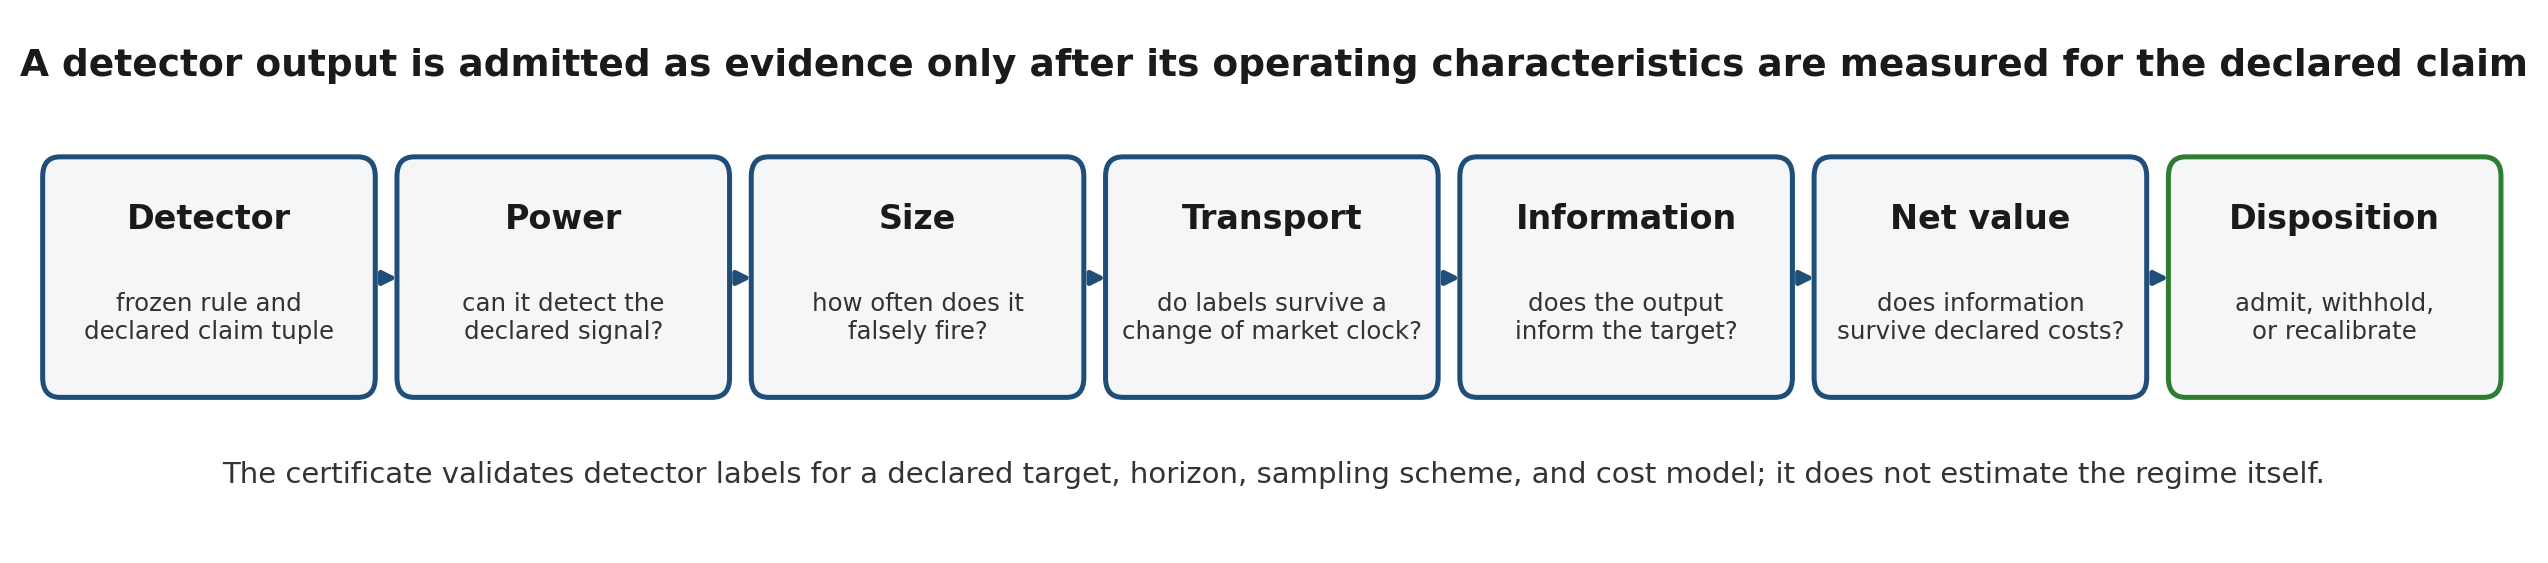
\includegraphics[width=\textwidth]{fig00_certification_pipeline.png}
\caption{Certification pipeline. A detector output is admitted as evidence
only after power, size, transport, information, and net-value gates have been
measured for the frozen claim tuple. The certificate validates detector
labels for a declared target, horizon, sampling scheme, and cost model; it
does not estimate the regime itself.}
\label{fig:pipeline}
\end{figure}

Section~\ref{sec:related} positions certification against the validation,
severity, data-snooping, market-clock, and information-value literatures.
Section~\ref{sec:method} defines the claim tuple, the gates, the certificate,
and the disposition rules. Section~\ref{sec:empirical} certifies the
variance-ratio cascade on BTCUSDT. Section~\ref{sec:families} runs three
detector families through the same protocol. Section~\ref{sec:discussion}
develops what certification adds relative to comparison testing, and
Section~\ref{sec:validity} states the domain of validity and the sequential
extension. Appendices contain derivations, the ETHUSDT replication, the
EUR/USD cost instantiation, and the reproducibility package.

\section{Positioning and Related Work}
\label{sec:related}

\subsection{Validation before use}

The nearest methodological ancestor of certification is the backtesting of
risk forecasts. \citet{Kupiec1995} tests whether a value-at-risk model's
violation frequency matches its nominal coverage; \citet{Christoffersen1998}
adds conditional coverage. Both are pre-use gates: a model whose violations
are mis-calibrated is not trusted, whatever its in-sample fit. Supervisory
model-risk guidance generalizes the posture---models require validation
commensurate with their use, ongoing monitoring, and explicit use
restrictions \citep{FederalReserveOCC2011}. Certification transfers this
discipline to regime detectors, whose outputs are neither forecasts nor
violation streams and therefore fall outside existing backtesting practice.
Three gates have no analogue in the VaR lineage and are the substance of the
transfer: power against a declared signal family, transport across sampling
schemes, and information value net of costs.

\subsection{Severity and the value of instrumented negatives}

The certificate's logic is the severity requirement of
\citet{Mayo2018} and \citet{MayoSpanos2006}: evidence counts only when
produced by a procedure with a demonstrated capacity to have found the claim
false. In our setting the demonstration is literal---known-amplitude signals
are injected into the empirical path and the detector's recovery probability
is measured. The inferential payoff is that non-detection becomes
quantitative: ``the detector was silent'' becomes ``the detector was silent,
and it detects $\delta=0.15$ departures with probability one at this horizon,
so amplitudes above $0.15$ are excluded.'' This is the minimum-detectable-effect
reporting format standard in experimental sciences, and it is what makes
negative results publishable evidence rather than absence of evidence
\citep{Harvey2017,HouXueZhang2020}. Signal injection as an instrument-calibration
device has a developed engineering practice in gravitational-wave detection
\citep{Biwer2017}; we import the practice, not the physics.

\subsection{What certification is not---and the gaps it closes}
\label{sec:not-comparison}

A large literature controls data-snooping when many rules are compared on one
sample: the reality check \citep{White2000}, stepwise extensions
\citep{RomanoWolf2005}, superior predictive ability \citep{Hansen2005}, the
model confidence set \citep{HansenLundeNason2011}, and their applications to
trading rules \citep{SullivanTimmermannWhite1999}. Multiple-testing discipline
for anomaly discovery makes the same point at the scale of the literature
itself \citep{HarveyLiuZhu2016,Bailey2016}. These methods answer a
\emph{relative} question---does the best of a universe beat a benchmark, and
which candidates are statistically indistinguishable from the best---and they
presuppose that each candidate's output is a valid measurement of a common
object. Certification answers the prior, \emph{absolute} question for a
single output and a single claim: is this label stream a valid measurement at
all, for this target, at this horizon, under this sampling scheme and cost
model? The two are complements, not substitutes: a detector can enter a model
confidence set while its labels fail transport certification, and a
certification pass says nothing about relative performance
(Section~\ref{sec:discussion} develops the contrast on our own artifacts).

No component check below is new, and the paper claims no novelty for power
curves, resampled nulls, equivalence tests, or information bounds. Run
separately, however, the components leave three gaps. First, there is no
single pre-declared object that ties detector, target, sampling scheme,
signal family, null family, cost model, and horizon together before evidence
is interpreted, so each check can be (and in practice is) run under silently
different conditions. Second, there is no precedence rule for multiple
failures---for example, a sensitive detector that is transport-uncertified
and cost-dominated---so ad hoc narratives fill the gap. Third, there is no
auditable output that tells a downstream user whether the detector may speak
for the claim at hand, must abstain, or must be recalibrated. The certificate
closes all three, and the closure has bite: several of our findings (the
uniform silence of the preregistered power grid, the horizon-discriminating
transport verdict, the convention-dependence of the value gate) are visible
only when the components are forced to share one frozen claim.

\subsection{Sampling schemes and market clocks}

That the sampling scheme is part of the measurement, not a nuisance choice,
is an old point in market microstructure: transaction, volume, and
subordinated clocks change the distributional properties of returns
\citep{MandelbrotTaylor1967,Clark1973,AneGeman2000,Guillaume1997,Dacorogna2001,Easley2012}.
A detector calibrated on calendar bars is therefore not automatically
portable to volume or event-time bars. Certification treats portability as a
statistical hypothesis to be certified---practical equivalence of a declared
output statistic within a preregistered margin \citep{Schuirmann1987}, with
multiplicity control \citep{Holm1979}---rather than as an assumption. We use
``transport'' in the spirit of the transportability literature, which asks
when results carry from one data-generating environment to another
\citep{PearlBareinboim2014}; here the environments are bar-construction
schemes over the same market history. An event-time (intrinsic) clock
advances when a pre-declared market movement or activity event occurs;
horizons are aligned across schemes by a declared calibration table before
any comparison is made.

\subsection{Information value and its ceiling}

The economic reading of detector output uses the growth-optimal bound: side
information about a payoff-relevant target raises attainable log-growth by at
most the mutual information between signal and target
\citep{Kelly1956,AlgoetCover1988,BarronCover1988,CoverThomas2006}. Two
disciplines follow. First, the relevant estimand is the information in the
\emph{detector output}, $I(D;Y)$, not the information in the raw path: by
data processing, a causal output cannot exceed the history it compresses, so
raw-path information is a scale diagnostic, never detector evidence. Second,
an upper bound net of costs is a use gate, not a performance claim: the
volatility-timing literature shows that economic value claims live or die on
cost and implementation assumptions \citep{MoreiraMuir2017,Cederburg2020},
and the certificate makes the cost convention an explicit, frozen field.

\subsection{Abstention, calibration, and certificates}

Certification's refusal states have counterparts in selective prediction and
classification-with-rejection, where a model abstains when its output is not
trustworthy \citep{GeifmanElYaniv2017}, in conformal prediction's validity
guarantees \citep{Vovk2005}, and in the calibration literature's insistence
that confidence match frequency \citep{Guo2017}. Machine-learning governance
has converged on structured pre-use disclosure documents---model cards
reporting a model's evaluation conditions and intended-use boundaries
\citep{Mitchell2019}---and measurement science supplies the reporting form
itself: an instrument is accompanied by a calibration certificate stating
what was measured, under what conditions, with what uncertainty, and with
what validity limits \citep{JCGM2008}. The detector certificate is that form,
instantiated for statistical instruments, with the difference that its fields
are measured gates with decision consequences rather than descriptive
disclosures.

\section{The Certification Protocol}
\label{sec:method}

\subsection{Claim tuple and operator}

Let a detector-output claim be
\[
  \mathcal{A} =
  (D_\theta,\, Y,\, g,\, W,\, q,\, s,\, \mathbb{P}_0^\ast,\, \epsg,\, Q,\, \crt),
\]
where $D_\theta$ is a frozen detector, $Y$ is the forward scientific or
economic target, $g$ is the sampling scheme (market clock), $(W,q)$ defines
the detector window and horizon, $s$ is the declared signal family,
$\mathbb{P}_0^\ast$ is the empirical null family, $\epsg$ is the
transport-equivalence margin, and $(Q,\crt)$ define the decision size and
cost model. Certification is the operator
\[
  \mathcal{O}(\mathcal{A})
  =
  (C_D,\ \mathrm{disposition},\ \mathrm{failure\ profile}),
  \qquad
  C_D=\{\Pdet,\ \alpha_D^\ast,\ \Delta_D,\ I_D,\ W_D\},
\]
mapping the claim to a measured characterization vector---power
($\Pdet$), empirical size ($\alpha_D^\ast$), transport discrepancy
($\Delta_D$), detector-output information ($I_D$), and net information value
($W_D$)---plus a disposition and a gate-level failure profile. Throughout,
``admissible'' is used in the evidentiary sense---whether an output may be
used as evidence for the declared claim---not in the decision-theoretic sense
of Wald; and ``net information value'' is a cost-adjusted Kelly-growth bound,
not the expected value of information of decision analysis. The detector
family is unrestricted: classical test statistics, state-space filters,
volatility rules, or learned classifiers are all admissible arguments, because
the operator evaluates outputs, not internals.

The operator runs seven stages on the frozen tuple: \emph{freeze} (fix all
tuple fields and record the commit), then the five measurement gates
\emph{power} $\Pdet$, \emph{size} $\alpha_D^\ast$, \emph{transport}
$\Delta_D$, \emph{information} $I_D$, and \emph{net value} $W_D$ defined
below, and finally a \emph{disposition} with its failure profile.
Figure~\ref{fig:pipeline} shows the ordering.

\subsection{Certificate, governance, and precedence}

A certification run produces a certificate rather than a scalar score;
Table~\ref{tab:certificate} lists the minimum fields. The claim owner---study
author or preregistration owner in research; model owner plus validation,
risk, and execution stakeholders in production---must freeze the tuple before
the output is used. Any change in detector code, target, bar construction,
venue, fee schedule, or market-structure condition triggers recertification
or an explicit monitoring exception.

\begin{table}[htbp]
\centering
\caption{Minimum certificate fields.}
\label{tab:certificate}
\small
\begin{tabularx}{\textwidth}{@{}lX@{}}
\toprule
Field & Required content \\
\midrule
Claim tuple & Frozen detector, target $Y$, sampling scheme $g$, horizon $(W,q)$, signal family $s$, null family, equivalence margin, decision size, cost model, and cost-attribution convention. \\
Power & Executed grid, draws per cell, fire rates, exact intervals, and response thresholds or explicit brackets; confirmatory versus exploratory provenance per cell. \\
Size & Null families, block or resampling parameters, number of draws $B$, Monte Carlo resolution at $B$, empirical false-alarm estimate, and the calibration of the nominal reference. \\
Transport & Statistics $\Phi$, scheme pairs, margin rationale, multiplicity adjustment, per-pair certification status, and precision limits of non-certified rows. \\
Information/value & Detector output used, target, estimator, uncertainty and permutation reference, and net value under the declared convention (with sensitivity to the attribution convention reported). \\
Failure profile & Gate-level reasons for non-admission, in precedence order, with all failed gates retained. \\
Governance & Certificate owner, artifact hashes or paths, freeze commit, expiry conditions, recalibration triggers, and downstream action. \\
\bottomrule
\end{tabularx}
\end{table}

Disposition precedence is conservative and fixed in advance by the following
rule, applied mechanically:
\begin{enumerate}[leftmargin=2.2em,itemsep=0.15em]
\item \emph{Instrument validity}: if frozen validity gates fail, the
disposition is \emph{instrument-failed} and no statistical gate is
interpreted.
\item \emph{Target eligibility}: if the detector measures a different object
than the claim target, the disposition is \emph{target-mismatched}.
\item \emph{Size}: if empirical false-alarm behavior is inconsistent with the
declared level (in either direction), the disposition is
\emph{size-distorted}.
\item \emph{Transport}: for transported claims, if required equivalence is
not certified, the disposition is \emph{transport-uncertified}.
\item \emph{Power}: if $\Pdet$ does not reach the required level on the
declared amplitude family, the disposition is \emph{underpowered}.
\item \emph{Information/value}: if $I_D$ is statistically unsupported or
$W_D\le0$ under the declared convention, the disposition is
\emph{cost-dominated}.
\end{enumerate}
Missing required estimands yield \emph{incomplete} unless the available
evidence already fails a gate above, in which case that gate's disposition is
reported and the missing coverage is recorded in the failure profile. When
several gates fail, the certificate reports the first failure in this order
and retains the rest in the profile. Every disposition in this paper,
including the exhibits of Sections~\ref{sec:empirical}
and~\ref{sec:families}, is generated by this rule. ``Admissible'' always
means admissible \emph{for this claim tuple}---never profitable, never
generally valid.

\subsection{Objects and gates}

Let $X=(r_1,\ldots,r_T)$ be an empirical return path. A sampling scheme
$g\in\mathcal{G}$ maps the same market history into a scheme-specific bar
path $T_g(X)$; in the demonstration $\mathcal{G}$ contains calendar, volume,
and event-time bars. A frozen detector is a causal map
$D_\theta(T_g(X)) \mapsto (F_t^g,L_t^g,S_t^g,M_t^g)$: trigger stream, label
stream, output statistic, and validity metadata, with $\theta$ frozen before
characterization. For a signal family $s$ and amplitude $\delta$, an
injection operator $J_{\delta,s}$ produces a perturbed empirical path; the
detector runs unchanged on the transformed, injected path.

\paragraph{Power.} The central estimand is
\begin{equation}
  \Pdet(\delta;W,q,g,s)
  =
  \Pr\{D_\theta(T_g(J_{\delta,s}(X)))\ \text{fires}\},
  \label{eq:pdet}
\end{equation}
with response thresholds
$\delta_p=\inf\{\delta : \Pdet(\delta;\cdot)\ge p\}$ for declared $p$
(here $p\in\{0.50,0.90\}$). We name $\delta_{90}$ the \emph{certified minimum
detectable effect} (cMDE): the smallest declared-family amplitude the frozen
detector recovers with probability at least $0.90$, on this asset, frequency,
horizon, and sampling scheme. The cMDE is intended as a portable reporting
primitive---the power analogue of a value-at-risk exception rate---so that
``detector $D$ has $\mathrm{cMDE}=0.15$ at $(q{=}2, \text{1-min BTCUSDT})$''
becomes a comparable, citable statement of instrument sensitivity, and a
negative result acquires a severity: departures above the cMDE are excluded
with demonstrated power, departures below it are not claimed either way. When
the executed grid does not identify $\delta_{90}$, the certificate reports a
bracket, never an extrapolation, and a cMDE from post-freeze amplitudes is
labeled exploratory-grade until a preregistered confirmatory rerun.

\begin{proposition}[Power-surface estimation]
\label{prop:power}
For a fixed detector rule, scheme, injection family, and grid cell, Monte
Carlo injection outcomes are Bernoulli draws with success probability
$\Pdet$. The sample fire rate estimates the response surface conditional on
the empirical path and injection design, and exact binomial intervals give
the finite-draw uncertainty.
\end{proposition}

The proposition is deliberately conditional---it characterizes the frozen
instrument on the declared noise path and signal family, and claims no
unconditional market law. Proofs of this and the following statements are
immediate and collected in \ref{app:derivations}.

\paragraph{Size.} Asymptotic references can fail in high-frequency data with
heavy tails, volatility clustering, and overlapping-window aggregation.
Certification therefore measures
\begin{equation}
  \alpha_D^\ast(W,q,g)
  =
  \Pr_{\mathbb{P}_0^\ast}\{D_\theta(T_g(X^\ast))\ \text{fires}\},
  \label{eq:size}
\end{equation}
under dependence-preserving nulls (circular block, stationary block, wild, or
sign-symmetric resampling; \citealp{Kunsch1989,PolitisRomano1994}). The
certificate must declare the draw budget $B$ and report the exact binomial
resolution at that budget; a low-$B$ diagnostic can demonstrate the gate but
cannot certify size for deployment. Size distortion in either direction is
reportable: an over-sized rule invalidates positives, and a strongly
conservative rule silently destroys power---a fact the power gate will
independently register.

\paragraph{Transport.} For a declared output statistic $\Phi$ and scheme pair
$(g,h)$, the transport discrepancy is
\begin{equation}
  \Delta_D(g,h;\Phi)
  =
  \bigl|\Phi(D_\theta(T_g(X))) - \Phi(D_\theta(T_h(X)))\bigr|,
  \label{eq:transport}
\end{equation}
and portability is certified only if two one-sided equivalence tests place
$\Delta_D$ inside the preregistered margin $\epsg$ after multiplicity control
across the declared family of pairs and horizons
\citep{Schuirmann1987,Holm1979}.

\begin{proposition}[Transport non-certification]
\label{prop:transport}
If practical equivalence is not certified for a pre-declared statistic
$\Phi$, then detector claims calibrated under scheme $g$ are not certified
under scheme $h$ without recalibration or a scheme-specific certificate.
\end{proposition}

Non-certification is not a demonstration of difference: a pair can fail
because the estimated discrepancy exceeds the margin or because the
comparison lacks precision (event-time bars are far scarcer than calendar
bars). The certificate distinguishes the two by reporting the interval
against the margin.

\paragraph{Information and net value.} Let $Y_{t+q}$ be the declared target
and $D_t^g$ the detector output available before the decision. The gate
estimand is the detector-output information
\begin{equation}
  I_D(q,g)=I(D_t^g;Y_{t+q}),
  \label{eq:id}
\end{equation}
never a raw-path quantity such as $I(\operatorname{sign} r_t;\operatorname{sign} r_{t+q})$.
For decision size $Q$ and all-in round-trip cost $\crt(q,Q,g)$, the net
information value in basis points per decision epoch is
\begin{equation}
  W_D(q,Q,g)=10{,}000\, I_D(q,g) - \crt(q,Q,g)\cdot \rho,
  \label{eq:wd}
\end{equation}
where $I_D$ is in nats under the log-optimal fair-odds bound
\citep{Kelly1956,AlgoetCover1988,CoverThomas2006} and $\rho$ encodes the
declared cost-attribution convention: under \emph{per-epoch} attribution
every decision epoch bears the full round-trip cost ($\rho=1$); under
\emph{per-trigger} attribution cost is borne only when the detector's action
state is on, so $\rho$ equals the trigger rate.
The conversion is an idealized gross upper bound on log-growth, not a
realized-profit forecast, and the cost term must include commissions, spread,
slippage, impact, funding, latency, and non-fill risk where relevant.
Equation~\eqref{eq:wd} makes the convention a certificate field because, as
Section~\ref{sec:empirical} shows, the sign of $W_D$ can depend on it.

\begin{proposition}[Cost gate]
\label{prop:cost}
If $W_D(q,Q,g)\le 0$ under the declared convention, detector-only use is
excluded for the stated target and cost model. $W_D>0$ is necessary but not
sufficient for economic use: it is an upper bound on attainable growth, not
an attainable strategy.
\end{proposition}

\begin{corollary}[Data-processing ceiling]
\label{cor:dpi}
If $D_t^g$ is a causal function of observed history,
$I(D_t^g;Y_{t+q})\le I(X_{\le t}^g;Y_{t+q})$: a detector output cannot be
credited with information that is only present in the raw history it
compresses.
\end{corollary}

\subsection{Certificate-level error control via e-values}
\label{sec:evalue}

The gates that are hypothesis tests---size, transport equivalence, and
information---admit a common error currency that the power and value
estimation gates do not require: the e-value. An e-value for a null $H_0$ is
a nonnegative statistic $E$ with $\mathbb{E}_{H_0}[E]\le 1$; by Markov's
inequality $\Pr_{H_0}(E\ge 1/\alpha)\le\alpha$, so certifying a gate at level
$\alpha$ means observing $E\ge 1/\alpha$ \citep{VovkWang2021,GrunwaldHeideCanonne2024}.
Writing each testing gate $k$ as an e-value $E_k$ for its inadmissibility
null $H_0^k$ turns the certificate's conjunction of gates into a single
error-controlled object.

\begin{proposition}[Static admission control, no multiplicity penalty]
\label{prop:static-e}
Suppose admission requires certifying every required testing gate,
$E_k\ge 1/\alpha$ for all $k\in K$. Under the global inadmissibility null
$H_0=\bigcup_{k\in K} H_0^k$ (the detector violates at least one gate),
$\Pr_{H_0}(\text{admit})\le\alpha$, with no correction for the number of
gates.
\end{proposition}

\begin{proposition}[Anytime-valid admission control]
\label{prop:online-e}
Suppose each gate is monitored by an e-process $(E^k_t)_{t\ge0}$---a
nonnegative supermartingale under $H_0^k$ with $\mathbb{E}[E^k_0]\le1$---and
admission at time $t$ requires $E^k_t\ge1/\alpha$ for all $k$. Then over an
unbounded monitoring horizon and any data-dependent stopping rule,
$\Pr_{H_0}(\exists\, t:\text{admit})\le\alpha$.
\end{proposition}

Proofs are in \ref{app:derivations}. Proposition~\ref{prop:static-e} is the
e-value form of the intersection--union test \citep{Berger1982}, of which the
transport TOST gate is the textbook case; the free multiplicity follows
because admission is a conjunction, so the worst case is governed by the
single hardest gate. Proposition~\ref{prop:online-e} is Ville's inequality
applied to the failing gate's e-process. Together they replace the fixed
error budget split across gates and the per-window maximum-statistic
multiplicity of a p-value monitor with one bound that holds continuously,
under optional stopping---the property a repeatedly consulted p-value monitor
lacks \citep{Ramdas2023}. For downstream propagation the certificate reports
the product $\prod_k E_k$ when gate e-values are built on separate data folds
and the average $|K|^{-1}\sum_k E_k$ otherwise, the latter an e-value under
arbitrary dependence.

The information gate instantiates this empirically. Its permutation
p-values calibrate to e-values through the a-priori calibrator
$f_\kappa(p)=\kappa p^{\kappa-1}$ at $\kappa=\tfrac12$, giving $E=2.17$ at
$q{=}2$ ($p=0.053$) and $E=15.8$ at $q{=}5$ ($p=0.001$); both fall short of
the $1/\alpha=20$ admission threshold at $\alpha=0.05$, the conservative
price of a distribution-free calibration. The deployment form is tighter and
unifies two gates: a sequential bettor staking the detector's forward-sign
prediction accumulates wealth that is an e-process for independence, and
whose log-growth rate is exactly the Kelly quantity of the value gate
$W_D$---so the information gate's evidence and its economic value are one
object viewed two ways.

\subsection{Run integrity}
\label{sec:integrity}

Certification is only as credible as its bookkeeping, so the protocol imports
reproducibility controls as inferential requirements, not engineering
conveniences. The claim tuple is frozen in a version-controlled
preregistration commit; every artifact records that commit, its own code
commit, and its random seeds; evidence produced after the freeze must carry
an explicit exploratory flag in its provenance block, and the certificate
must disclose that flag wherever the evidence is displayed; data outside the
declared development span is excluded by the loader, and each artifact
records the exclusion flag. Each of these controls is engaged---and its
consequences disclosed---by the demonstration in
Section~\ref{sec:empirical}.

\section{Certifying a Variance-Ratio Cascade on BTCUSDT}
\label{sec:empirical}

\subsection{Data, detector, and declared claim}

The demonstration uses BTCUSDT one-minute perpetual futures over \dataspan\
($n=\numbars$ bars; effective span 2021-05-29 to 2025-12-31). The market is
treated as an empirical noise environment for instrument characterization,
not as the object of an efficiency claim. The worked detector is a
Holm-corrected Lo--MacKinlay variance-ratio cascade
\citep{LoMacKinlay1988,LoMacKinlay1989,Holm1979}: for horizon $q$, the
variance-ratio departure is computed from overlapping $q$-period returns
inside non-overlapping windows of width $W$; the cascade fires when at least
one horizon in $\{2,5,15,60\}$ has a Holm-adjusted two-sided p-value at or
below $0.05$ \emph{and} a positive median standardized statistic. The
positive sign gate makes the instrument a positive-autocorrelation trigger,
not a general $|\VR-1|$ detector. Multiple-horizon variance-ratio testing
otherwise follows the joint-testing lineage of \citet{ChowDenning1993}, with
finite-sample refinements available through rank/sign and wild-bootstrap
variants \citep{Wright2000,Kim2006}.

The declared claim to be certified is: \emph{the cascade's trigger stream may
be used as evidence of positive short-horizon serial dependence on
calendar-time bars---primary horizon $q{=}5$, window $W{=}120$---and its
triggers may be read economically under a $10$\,\bps\ all-in round-trip cost
convention at unit decision size.} The signal family $s$ is a positive AR(1)
injection calibrated to target $|\VR(q)-1|$ amplitudes; the null family is a
centered circular block bootstrap (block length $120$); the transport margin
is $\epsg=0.02$ on the median $|\VR-1|$ scale. The tuple was frozen in
preregistration commit \texttt{1dc5c82} (v4.0, 2026-06-11), with an earlier
v3.0 freeze lineage (2026-06-05) governing the holdout and replication runs;
all artifacts pin these commits and seed $43$.

\subsection{Power: a preregistered exclusion grid and disclosed positive controls}
\label{sec:power}

The preregistered power design is a 96-cell grid: amplitudes
$\delta\in\{0.0005,\allowbreak 0.001,\allowbreak 0.002,\allowbreak 0.005,\allowbreak 0.01,\allowbreak 0.02,\allowbreak 0.05,\allowbreak 0.10\}$, horizons
$q\in\{2,5,15,60\}$, windows $W\in\{60,120,240\}$, with $200$ Monte Carlo
injection draws per cell. The confirmatory result is uniform: \emph{in all 96
preregistered cells the cascade fired on 0 of 200 draws}
($\widehat{\Pdet}=0$, exact 95\% interval $[0,0.0182]$ per cell). In
minimum-detectable-effect form: for this detector class, injection design,
and noise path, detection of variance-ratio departures $\delta\le 0.10$ is
excluded at every tested window--horizon combination, with per-cell fire
probability bounded above by $1.8\%$ at 95\% confidence.

After the freeze, eight additional cells were run at larger amplitudes as
positive controls. Their provenance blocks carry an explicit exploratory
flag, and we report them as exploratory evidence, separately from the
confirmatory grid (Table~\ref{tab:power}). They establish that the harness
detects large signals---$\delta=0.15$ at $q{=}2$ fires on every draw at all
three windows---and they bracket the response thresholds:
$\delta_{90}(q{=}2)\in(0.10,0.15]$ for all tested $W$;
$\delta_{90}(q{=}5,W{=}120)\in(0.20,0.30]$; at $q{=}5$ with $W\in\{60,240\}$
the threshold exceeds $0.15$ and is unbracketed above on the executed grid;
at $q\in\{15,60\}$ it exceeds $0.10$ and is unbracketed. Because the
bracketing amplitudes were executed post-freeze, these brackets are
exploratory-grade: a certificate-grade threshold statement requires a
post-registered confirmatory rerun at the bracketing amplitudes. The design
lesson is recorded rather than hidden: a confirmatory amplitude grid should
be frozen only after a pilot power scan brackets the response region, which
the v4.0 design did not do---the addendum exists because of that gap, and the
disclosure obligation is the protocol registering its own design debt. Under
the declared claim---whose scientifically interesting amplitudes lie at or
below $0.10$---the instrument is \emph{underpowered}: the observed market
departure at the primary cell (median $|\VR(5)-1|=0.1603$) sits between the
excluded region and the $q{=}5$ response threshold, in a range where the
cascade has never demonstrated recovery.

\begin{table}[htbp]
\centering
\begin{threeparttable}
\caption{Power gate. Confirmatory grid (preregistered, freeze
\texttt{1dc5c82}) and exploratory positive controls (post-freeze,
\texttt{exploratory\_addendum: true} in artifact provenance). All cells use
200 draws; intervals are exact Clopper--Pearson 95\%.}
\label{tab:power}
\small
\begin{tabular}{l l c c c}
\toprule
Provenance & Cells & Fires / draws & $\widehat{\Pdet}$ & 95\% interval \\
\midrule
Confirmatory & all 96: $\delta\le 0.10$, $q\in\{2,5,15,60\}$, $W\in\{60,120,240\}$ & 0 / 200 each & 0.00 & $[0.0000, 0.0182]$ \\
\midrule
Exploratory & $\delta=0.15$, $q=2$, $W\in\{60,120,240\}$ & 200 / 200 each & 1.00 & $[0.9818, 1.0000]$ \\
Exploratory & $\delta=0.15$, $q=5$, $W\in\{60,120,240\}$ & 0 / 200 each & 0.00 & $[0.0000, 0.0182]$ \\
Exploratory & $\delta=0.20$, $q=5$, $W=120$ & 0 / 200 & 0.00 & $[0.0000, 0.0182]$ \\
Exploratory & $\delta=0.30$, $q=5$, $W=120$ & 200 / 200 & 1.00 & $[0.9818, 1.0000]$ \\
\bottomrule
\end{tabular}
\begin{tablenotes}\footnotesize
\item Response-threshold brackets implied by the executed grid:
$\delta_{90}(q{=}2,\cdot)\in(0.10,0.15]$;
$\delta_{90}(q{=}5,W{=}120)\in(0.20,0.30]$;
$\delta_{90}(q{=}5,W\in\{60,240\})>0.15$;
$\delta_{90}(q\in\{15,60\},\cdot)>0.10$. No interpolation is performed.
\end{tablenotes}
\end{threeparttable}
\end{table}

\begin{figure}[htbp]
\centering
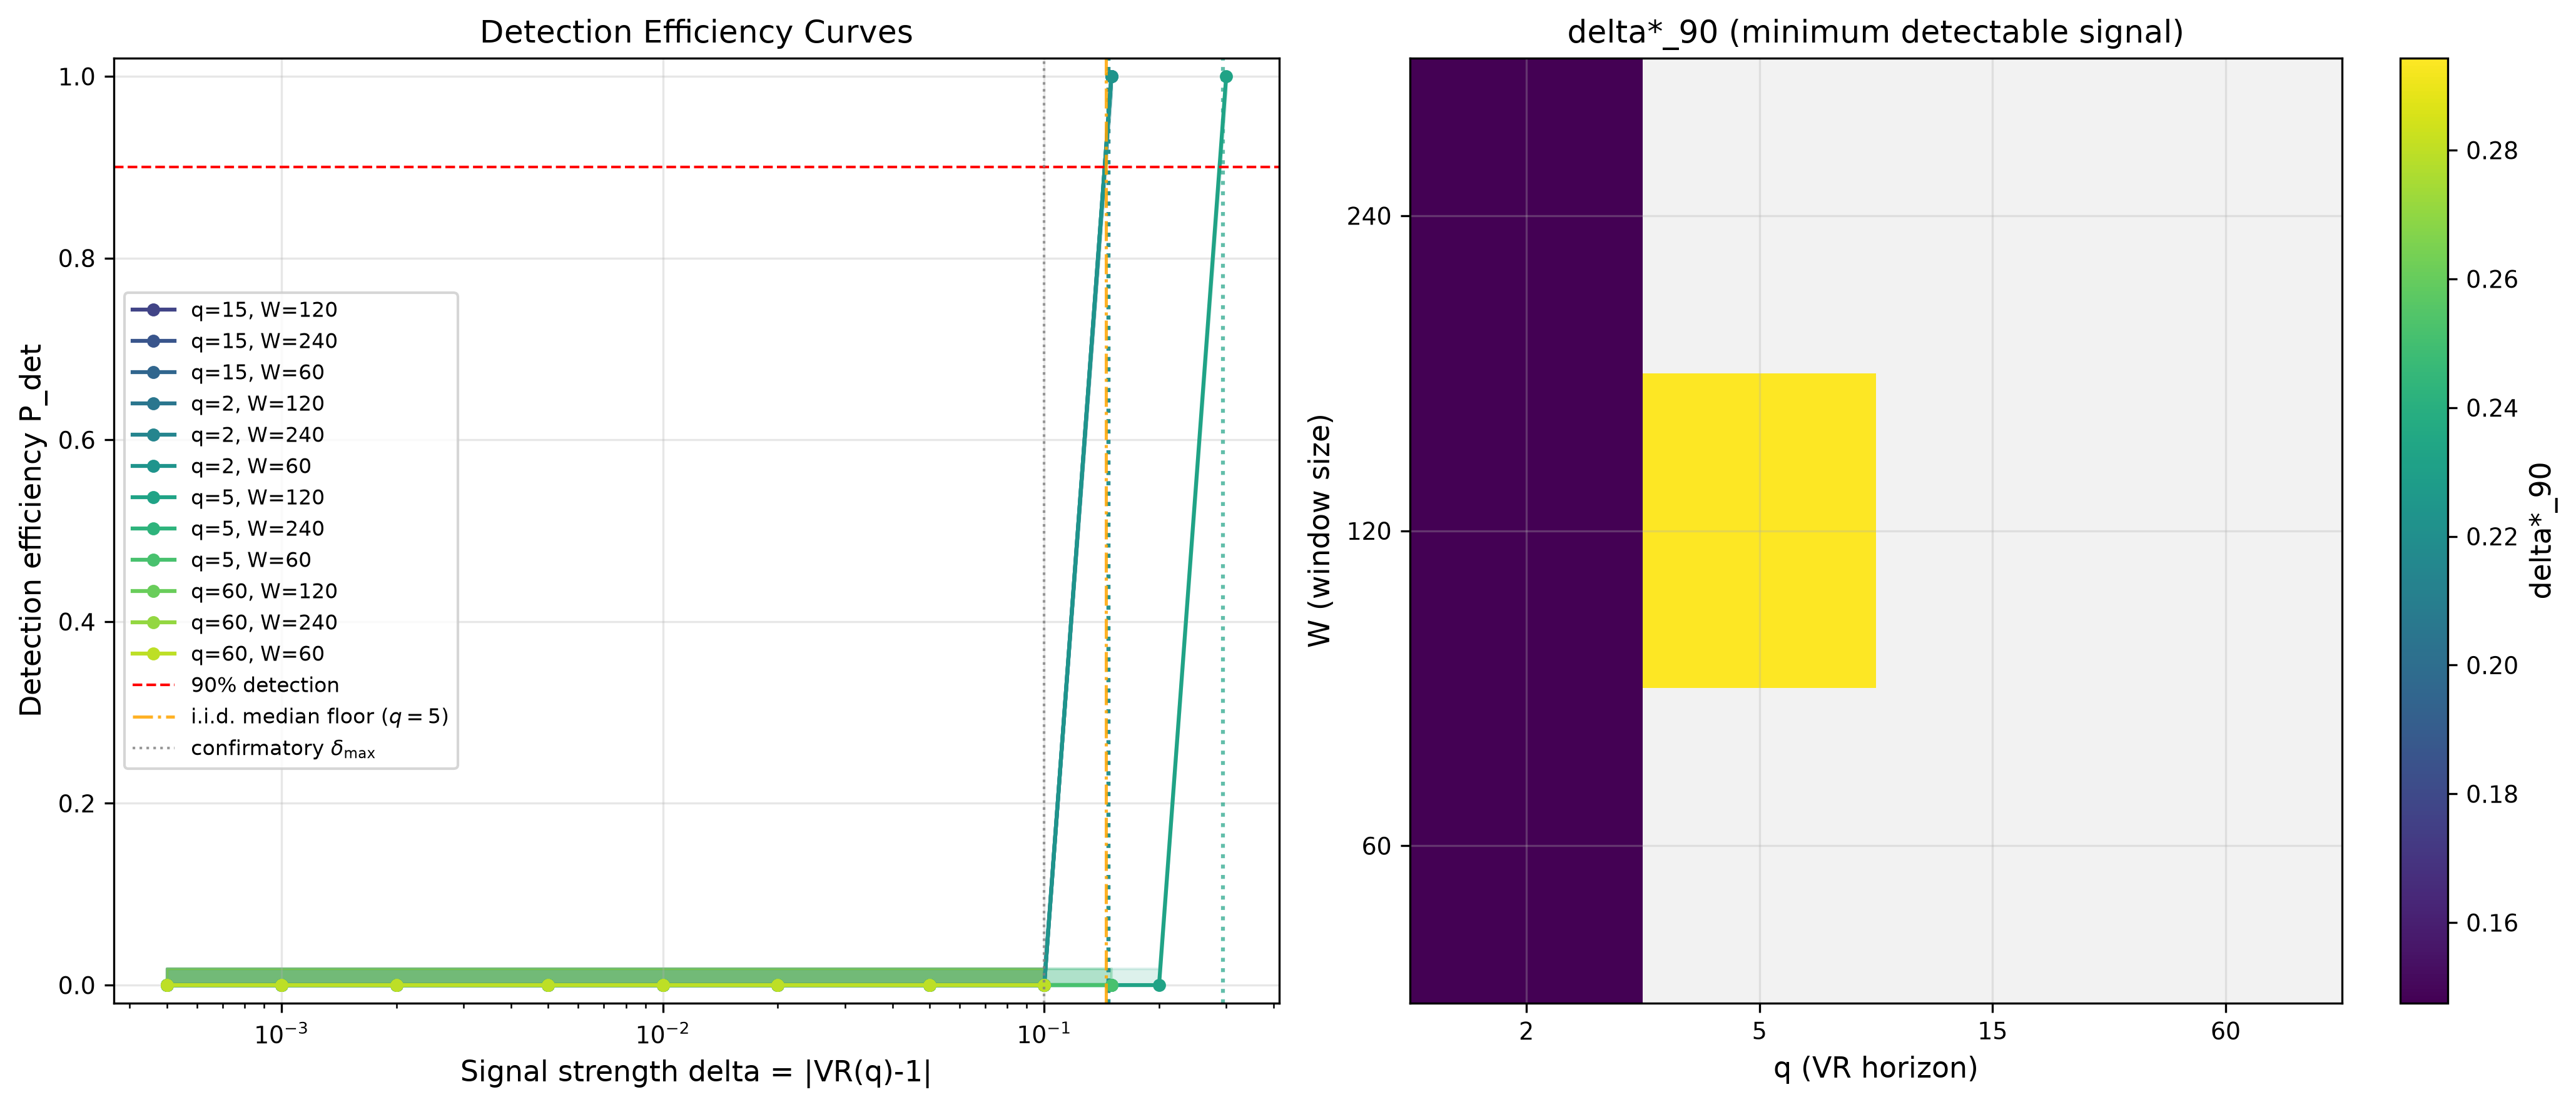
\includegraphics[width=0.85\textwidth]{fig01_exclusion.png}
\caption{Power surface for the frozen cascade. Left: fire rate against
injected amplitude for all twelve $(q,W)$ combinations; every preregistered
cell ($\delta\le0.10$, dotted vertical line) is at zero, and the rise to
certain detection occurs only in the exploratory region ($q{=}2$ at
$\delta=0.15$; $q{=}5$, $W{=}120$ at $\delta=0.30$). Right: implied
$\delta_{90}$ where the executed grid identifies it; grey cells are
unbracketed above. The step from 0/200 to 200/200 between adjacent executed
amplitudes reflects the grid resolution, not a measured discontinuity.}
\label{fig:power}
\end{figure}

The sharpness of the transition---0/200 at one executed amplitude, 200/200 at
the next---is a property of the cascade's aggregated decision statistic
discussed next, and the size gate explains why the thresholds are as high as
they are.

\subsection{Size: empirical false-alarm behavior and reference calibration}
\label{sec:size}

The size gate was audited at the two cascade-relevant cells
($W{=}120$, $q\in\{2,5\}$) under a centered circular block bootstrap of the
full return path (block length 120, $B=100$, seed 43). Two findings.

First, the false-alarm estimate: at nominal level $0.05$, the asymptotic
two-sided rule fired on \emph{0 of 100} null replicates in both audited
cells ($\widehat{\alpha}_D^\ast=0$, exact 95\% interval $[0,0.0362]$). Since
the interval excludes the nominal $0.05$, the empirical level is
significantly below nominal: by gate~3 of the precedence rule
(Section~\ref{sec:method}) this is a certified \emph{size distortion in the
conservative direction}, not a pass. Two scope caveats are part of the finding. The audit covers the two
cascade-relevant per-horizon cells, not the four-horizon union rule; the
full-cascade false-alarm rate on the same 100 resampled paths is a required
extension for a deployment certificate. And the executed null is a single
dependence-preserving family; the wild-bootstrap null, which imposes the
martingale-difference hypothesis the variance-ratio statistic actually tests
\citep{Kim2006}, is part of the declared certificate-grade family and was
not run at this diagnostic budget.

Second, the reference calibration: the cascade aggregates window-level
standardized statistics into a median, and the artifact records where that
median actually lives under the dependence-preserving null---centered at
$-0.165$ ($q{=}2$) and $-0.389$ ($q{=}5$), with 5th--95th percentile spans of
only $0.029$ and $0.023$ respectively. The $N(0,1)$ asymptotic reference used
by the frozen rule is therefore mis-centered and mis-scaled for this
aggregated statistic: the observed market medians ($-0.1819$ at $q{=}2$,
$-0.4017$ at $q{=}5$) receive asymptotic two-sided p-values of $0.856$ and
$0.688$, while their positions in the empirical null distribution give
$0.040$ and $0.050$ (both below the null 5th percentile; Holm-adjusted over
the two audited cells, $0.079$). Neither ingredient of this miscalibration is
mysterious after the fact: the negative center is the known finite-sample
bias of overlapping variance-ratio statistics \citep{LoMacKinlay1989}, and
the tight dispersion is what aggregating $\sim$$20{,}000$ window statistics
into a median produces. The gate's value is not discovery but registration:
the frozen rule shipped with a foreseeable miscalibration unhandled, and the
certificate records it against the rule rather than leaving it implicit in
the p-value formula. The direction also matters: both observed medians lie on
the \emph{negative} side, so the one-sided positive gate correctly withholds
(empirical positive-gate p-values $0.970$ and $0.960$), and no confirmatory
market claim arises from these cells.

\begin{table}[htbp]
\centering
\begin{threeparttable}
\caption{Size gate at the audited cells ($W{=}120$; centered circular block
bootstrap, block length 120, $B=100$).}
\label{tab:size}
\small
\begin{tabular}{c c c c c c c}
\toprule
$q$ & $\widehat{\alpha}_D^\ast$ (95\%) & Null median (p05, p50, p95) & Obs.\ median $Z$ & Asympt.\ p & Empir.\ p & Pos.-gate p \\
\midrule
2 & $0/100$ $[0,0.036]$ & $(-0.180, -0.165, -0.151)$ & $-0.1819$ & $0.856$ & $0.040$ & $0.970$ \\
5 & $0/100$ $[0,0.036]$ & $(-0.401, -0.389, -0.378)$ & $-0.4017$ & $0.688$ & $0.050$ & $0.960$ \\
\bottomrule
\end{tabular}
\begin{tablenotes}\footnotesize
\item $\widehat{\alpha}_D^\ast$: share of null replicates on which the
nominal-level asymptotic two-sided rule fired. ``Empir.\ p'': two-sided
position of the observed median in the null distribution of medians
(Holm-adjusted over the two audited cells: $0.079$ each). $n=20{,}126$
non-overlapping windows per replicate. A deployment certificate would rerun
this gate at the Monte Carlo budget declared in Table~\ref{tab:certificate};
$B=100$ demonstrates the gate and bounds, but does not resolve, the
false-alarm rate.
\end{tablenotes}
\end{threeparttable}
\end{table}

The size and power gates now explain each other, which is the point of
binding them in one certificate: a rule whose reference is mis-centered by
several null standard deviations in the conservative direction almost never
rejects---so its false-alarm rate is near zero \emph{and} its response
thresholds are far above the amplitudes of scientific interest. The
certificate records the pair as two consistent failures (size-distorted in
the conservative direction; underpowered below $\delta=0.15$), which is a
diagnosis, not a defense, of the frozen instrument.

\subsection{Transport: equivalence across calendar, volume, and event-time bars}
\label{sec:transport}

The transport gate compares the median $|\VR-1|$ departure across calendar
(clock), volume, and event-time (intrinsic) bar constructions of the same
market history, with horizons aligned by a frozen calibration table (median
bar durations: 1, 4, and 22 minutes respectively). Equivalence within
$\epsg=0.02$ is tested per scheme pair and horizon by two one-sided tests,
Holm-adjusted across the full 12-comparison family. Table~\ref{tab:transport}
reports every row; nothing is omitted.

\begin{table}[htbp]
\centering
\begin{threeparttable}
\caption{Transport gate, BTCUSDT \dataspan: all 12 preregistered
comparisons. Margin $\epsg=0.02$ on median $|\VR-1|$; 90\% intervals; Holm
over the 12-row family. ``Certified'' requires Holm-adjusted equivalence.}
\label{tab:transport}
\small
\begin{tabular}{c l c c c c}
\toprule
$q$ & Scheme pair & $\widehat{\Delta}_D$ & 90\% CI & Holm p & Certified \\
\midrule
2 & clock--volume & 0.0093 & [0.0068, 0.0118] & $1.8\times10^{-11}$ & yes \\
2 & clock--intrinsic & 0.0142 & [0.0105, 0.0179] & 0.0497 & yes \\
2 & volume--intrinsic & 0.0049 & [0.0007, 0.0090] & $1.2\times10^{-8}$ & yes \\
5 & clock--volume & 0.0231 & [0.0179, 0.0283] & 1.000 & no \\
5 & clock--intrinsic & 0.0351 & [0.0260, 0.0442] & 1.000 & no \\
5 & volume--intrinsic & 0.0120 & [0.0023, 0.0217] & 0.701 & no \\
15 & clock--volume & 0.0237 & [0.0163, 0.0312] & 1.000 & no \\
15 & clock--intrinsic & 0.0279 & [0.0007, 0.0550] & 1.000 & no \\
15 & volume--intrinsic & 0.0041 & [$-$0.0233, 0.0315] & 1.000 & no \\
60 & clock--volume & 0.0040 & [$-$0.0079, 0.0159] & 0.123 & no \\
60 & clock--intrinsic & 0.0014 & [$-$0.0278, 0.0306] & 1.000 & no \\
60 & volume--intrinsic & $-$0.0026 & [$-$0.0335, 0.0283] & 1.000 & no \\
\bottomrule
\end{tabular}
\begin{tablenotes}\footnotesize
\item Non-overlapping window counts at $q{=}5$, $W$-equivalent $120$: clock
$20{,}126$; volume $3{,}500$; intrinsic $454$. Rows whose interval width
exceeds the two-sided margin ($2\epsg=0.04$; e.g., all intrinsic pairs at
$q\ge15$) are precision-limited: equivalence could not have been certified
at any discrepancy, and non-certification there is an evidence statement,
not a difference finding. At $q{=}5$ the clock--volume and clock--intrinsic
point estimates exceed the margin itself. The $q{=}2$ clock--intrinsic
certification is marginal (Holm p $=0.0497$); the certified-at-$q{=}2$
headline does not hinge on it, but a certificate consumer should know.
\end{tablenotes}
\end{threeparttable}
\end{table}

\begin{figure}[htbp]
\centering
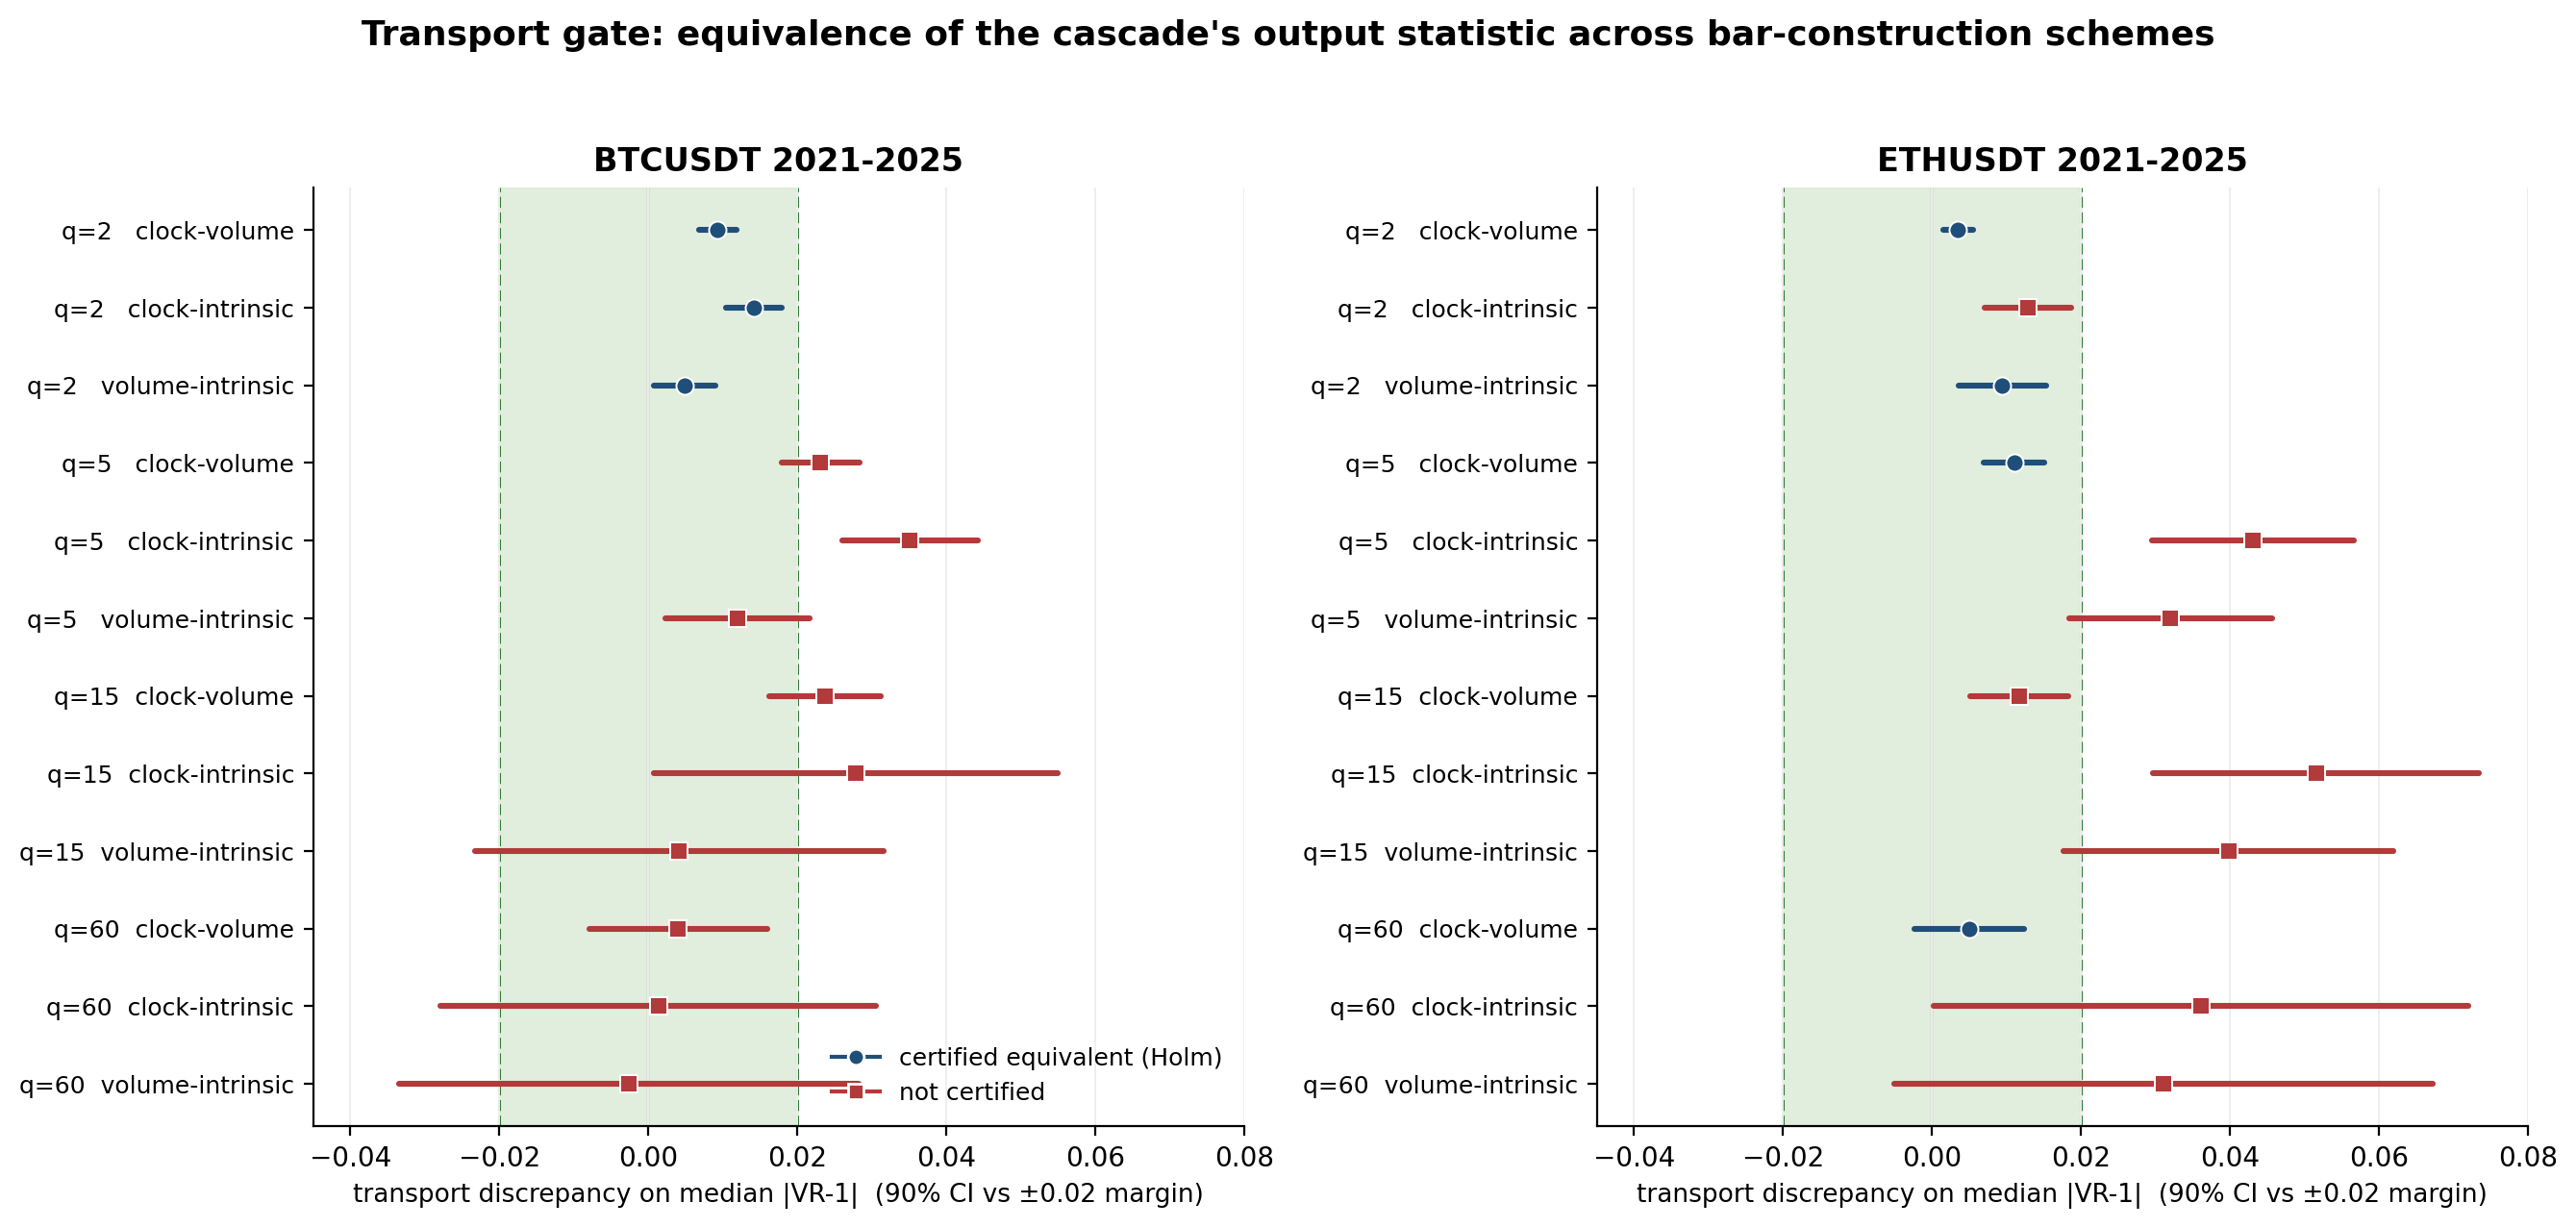
\includegraphics[width=\textwidth]{fig02_transport_forest.png}
\caption{Transport gate as an equivalence forest plot: 90\% intervals for the
transport discrepancy against the preregistered $\pm0.02$ margin (shaded),
BTCUSDT (left) and ETHUSDT (right). Certification requires Holm-adjusted
equivalence across the 12-row family, not merely an interval inside the
band---hence rows such as ETH $q{=}2$ clock--intrinsic (interval inside the
band, Holm p $=0.154$) and BTC $q{=}60$ clock--volume (Holm p $=0.123$)
remain uncertified: the multiplicity discipline binds.}
\label{fig:transport-forest}
\end{figure}

The verdict is horizon-specific (Figure~\ref{fig:transport-forest}). At
$q{=}2$ every scheme pair certifies: short-horizon cascade labels are
portable across all three bar constructions within the margin. At the primary
horizon $q{=}5$ no pair certifies, and the two clock-anchored discrepancies
exceed the margin outright---volume and event-time bars attenuate the
calendar-time departure (medians $0.160\to0.137\to0.125$). At $q\ge15$ the
event-time comparisons are precision-limited (454 windows). Under
Proposition~\ref{prop:transport}, the declared $q{=}5$ claim is
\emph{transport-uncertified}: calendar-bar labels are not certified evidence
about volume- or event-bar regimes at that horizon, while the same statement
at $q{=}2$ \emph{is} certified. The gate passes where bar construction is
immaterial and fails where it is material; the ETHUSDT replication
(\ref{app:eth}) repeats the pattern with a different certified set,
confirming that transport certification is an asset- and horizon-specific
measurement rather than a fixed property of the detector.

\subsection{Information and net value: the convention is load-bearing}
\label{sec:info}

The information gate estimates $I_D=I(D_t;\,\operatorname{sign} r_{t+q})$ for
the cascade's binary trigger on non-overlapping $W{=}120$ windows
($20{,}126$ labels), using the plug-in estimator on the $2\times2$
label--target table, with bootstrap intervals and a permutation reference
(Table~\ref{tab:info}). Two estimation caveats bound what these numbers can
support. The plug-in estimator's first-order (Miller--Madow) bias for a
$2\times2$ table is $1/(2n)\approx2.5\times10^{-5}$ nats upward---about
$0.25$\,\bps, i.e., a fifth of the $q{=}2$ estimate---so small positive
$I_D$ values should be read net of that order. And the permutation reference
shuffles label--target pairings, which imposes exchangeability at the window
scale; a block-permutation reference consistent with the certificate's own
dependence-preservation requirement is the certificate-grade instrument and
was not run at this budget. With those caveats, the triggers are
sparse---74 fires at $q{=}2$ (rate $0.0037$), 115 at $q{=}5$ (rate
$0.0057$)---and the information is resolvable at $q{=}5$
($I_D=3.46\times10^{-4}$ nats, permutation $p=0.001$) and marginal at
$q{=}2$ ($1.28\times10^{-4}$ nats, $p=0.053$). Raw sign-pair information on
the same data is recorded in the artifacts as a scale diagnostic only; by
Corollary~\ref{cor:dpi} it is never detector evidence, and we do not report
it as such.

\begin{table}[htbp]
\centering
\begin{threeparttable}
\caption{Information and net-value gates for the frozen cascade trigger.
Kelly conversion $10{,}000\cdot I_D$ (nats$\to$\bps); cost convention
$\crt=10$\,\bps\ round-trip at unit size.}
\label{tab:info}
\small
\begin{tabular}{c c c c c c c}
\toprule
$q$ & Triggers & $I_D$ (nats) & Perm.\ p & Gross bound & $W_D$ per-epoch & $W_D$ per-trigger \\
 & (of 20{,}126) & [95\% boot.] & & (\bps) & (\bps) & (\bps) \\
\midrule
2 & 74 & $1.28\times10^{-4}$ $[0.21, 4.46]\times10^{-4}$ & 0.053 & 1.28 & $-8.72$ & $+1.25$ \\
5 & 115 & $3.46\times10^{-4}$ $[0.38, 10.3]\times10^{-4}$ & 0.001 & 3.46 & $-6.54$ & $+3.41$ \\
\bottomrule
\end{tabular}
\begin{tablenotes}\footnotesize
\item Per-epoch: every decision epoch bears the full round-trip cost,
$W_D=10{,}000 I_D - \crt$. Per-trigger: cost is borne only on trigger
epochs, $W_D=10{,}000 I_D - \crt\times(\text{trigger rate})$; equivalently,
per trigger event the gross bound is $349$\,\bps\ ($q{=}2$) and $606$\,\bps\
($q{=}5$) against a $10$\,\bps\ round-trip. Conditional forward returns on
trigger epochs are negative on average ($-1.7\times10^{-4}$ at $q{=}2$,
positive fraction $0.38$), so the resolvable information is not a
directional long signal; the bound is direction-agnostic.
\end{tablenotes}
\end{threeparttable}
\end{table}

The net-value column is the methodological finding of this subsection: under
per-epoch attribution the trigger's information is dominated by the
$10$\,\bps\ convention ($W_D=-8.72$ and $-6.54$\,\bps), while under
per-trigger attribution the bound is positive ($+1.25$ and $+3.41$\,\bps\
per epoch). The two conventions have distinct semantics, not merely distinct
arithmetic: per-epoch attribution is the coherent reading for an always-on
state detector, and for a sparse trigger that implies action on
$0.4$--$0.6\%$ of epochs it is a deliberately conservative upper-cost
convention; per-trigger attribution matches the trigger's action semantics.
The frozen tuple declared per-epoch attribution ex ante, so the gate input
under the declared claim is \emph{cost-dominated}, with the per-trigger
sensitivity disclosed---and the lesson the certificate encodes is that the
convention must match the declared action semantics when the tuple is
frozen, because the verdict does not survive the substitution. Propagating
the bootstrap intervals through Equation~\eqref{eq:wd} bounds what either
verdict can claim: per-epoch $W_D$ at $q{=}2$ is resolved negative
($[-9.79,-5.54]$\,\bps) but at $q{=}5$ straddles zero
($[-9.62,+0.33]$\,\bps), so even the frozen-convention cost domination at
the primary horizon is a point-estimate statement, not a 95\%-resolved one;
per-trigger $W_D$ is positive across both intervals ($[+0.17,+4.42]$ and
$[+0.32,+10.28]$\,\bps). Proposition~\ref{prop:cost} caps what any positive
bound could license: an idealized fair-odds growth ceiling, not an attainable
strategy---and the trigger-conditional forward returns (negative mean on
trigger epochs, positive fraction $0.38$ at $q{=}2$) show the resolvable
information is not a simple directional long signal. For a state-type
detector that is always on, the two conventions coincide
(Section~\ref{sec:families}), so the convention field is load-bearing
precisely for sparse-trigger instruments.

\subsection{A temporally disjoint 2026 window}
\label{sec:holdout}

Data from 2026-01-01 to 2026-05-29 ($214{,}355$ bars; $1{,}786$
non-overlapping $W{=}120$ windows) were excluded from all development runs by
a loader-level exclusion flag recorded in every development artifact. On the
primary cell the cascade did not
fire: observed $|\VR(5)-1|=0.1575$ (mean $0.1835$), median standardized
statistic $-0.3328$, asymptotic two-sided p $=0.739$. The observed departure
again exceeds the frozen exclusion bound ($0.10$) while lying below the
demonstrated response threshold and on the negative side of the sign gate---
the same disposition pattern as in-sample. We label this window a
\emph{temporally disjoint evaluation block} rather than a prospective
holdout: the preregistration lineage (v3.0 amendment \texttt{dd44e7a},
2026-06-05; executed 2026-06-23) postdates the end of the window, so the
separation is enforced by the recorded loader flag and freeze discipline, not
by a third-party timestamp that predates the data. The distinction is
exactly the kind of provenance fact a certificate exists to carry.

\subsection{The completed certificate}
\label{sec:certificate-exhibit}

Table~\ref{tab:cert-filled} exhibits the certificate for the declared claim.
This table is the paper's central deliverable: every field is a measured
quantity with a frozen artifact behind it, and the disposition follows
mechanically from the precedence rule.

\begin{table}[htbp]
\centering
\begin{threeparttable}
\caption{Completed admissibility certificate: Holm-corrected VR cascade,
BTCUSDT \dataspan.}
\label{tab:cert-filled}
\small
\begin{tabularx}{\textwidth}{@{}lX@{}}
\toprule
Field & Certified content \\
\midrule
Claim tuple & Frozen cascade ($q$-grid $\{2,5,15,60\}$, Holm $0.05$, positive median gate); target: positive short-horizon serial dependence, economically read at $q{=}5$, $W{=}120$; scheme: calendar 1-min bars; signal family: positive AR(1) injections; null: centered circular block ($L{=}120$); $\epsg=0.02$; cost: $10$\,\bps\ round-trip, unit size, per-epoch attribution. Freeze \texttt{1dc5c82} (2026-06-11), seed 43. \\
Power & 96/96 preregistered cells silent at $\delta\le0.10$ (0/200 each, 95\% upper bound 0.0182). Exploratory brackets: $\delta_{90}(q{=}2)\in(0.10,0.15]$, $\delta_{90}(q{=}5,W{=}120)\in(0.20,0.30]$. \emph{Underpowered} for the declared amplitude family ($\delta\le0.10$). \\
Size & $\widehat{\alpha}_D^\ast=0/100$ $[0,0.036]$ at both audited cells; interval excludes nominal $0.05$; asymptotic reference mis-centered (null medians $-0.165$/$-0.389$, spans $<0.03$). \emph{Size-distorted, conservative direction}; $B=100$ resolution limit and single-null-family scope declared. \\
Transport & Certified at $q{=}2$ for all three scheme pairs (clock--intrinsic marginal, Holm $0.0497$); not certified at $q{=}5$ (clock-anchored discrepancies exceed $\epsg$); $q\ge15$ event-time rows precision-limited. \emph{Transport-uncertified} at the primary horizon. \\
Information/value & $I_D=3.46\times10^{-4}$ nats at $q{=}5$ (perm.\ $p=0.001$; plug-in bias order $0.25$\,\bps); $W_D=-6.54$\,\bps\ per-epoch (frozen convention; interval $[-9.62,+0.33]$ straddles zero) vs.\ $+3.41$\,\bps\ per-trigger; \emph{cost-dominated} under the frozen convention at the point estimate, convention- and interval-sensitivity disclosed. \\
Run integrity & All artifacts pin freeze/code commits and seeds; 2026 data loader-excluded in development (flag recorded); 8 post-freeze cells carry the exploratory provenance flag and are reported as exploratory. \\
Failure profile & Generated by the Section~\ref{sec:method} precedence rule: (3) size-distorted (conservative) $\rightarrow$ (4) transport-uncertified ($q{=}5$) $\rightarrow$ (5) underpowered (declared amplitudes $\delta\le0.10$) $\rightarrow$ (6) cost-dominated (frozen convention, point estimate). Gates (1)--(2) pass. \\
Disposition & \textbf{Withheld: size-distorted (conservative)}, with the full profile above. The same evidence supports two bounded instrument statements: $q{=}2$ labels are transport-certified across all three schemes, and the cascade \emph{cannot detect} departures $\delta\le0.10$ under this design (an instrument-scope statement; it admits no market claim about the existence or absence of dependence). \\
\bottomrule
\end{tabularx}
\end{threeparttable}
\end{table}

Non-detection has become a diagnostic vector rather than a generic failure:
the cascade is a conservative instrument whose reference needs recentering,
whose response threshold sits above the declared amplitudes, whose labels
transport at one horizon but not another, and whose trigger information is
real but convention-dependently valued. Each statement is bounded,
artifact-backed, and independently actionable---and the next subsection acts
on the first of them.

\subsection{The diagnosis is actionable: recentering and the first admissible
certificate}
\label{sec:repair}

A certificate that only ever refuses is of limited use; the test of the
protocol is whether its diagnoses repair the instrument. The size gate
localized the fault precisely: the decision statistic (the median window-level
$Z$) is referred to $N(0,1)$, but under the dependence-preserving null it is
centered near $-0.005$ ($q{=}2$) and $-0.106$ ($q{=}5$) with standard
deviation $\approx0.01$. We therefore replace the asymptotic reference with
an empirical-null reference---studentizing the statistic by the null center
and spread estimated from the $\delta\!=\!0.0005$ calibration cell and firing
one-sidedly on positive departures---and re-evaluate every gate. Because each
injection draw's per-horizon statistic is stored in the frozen artifacts, the
recentered rule is applied by exact offline re-thresholding of the same
$104\times200$ draws: no new simulation, no raw data, fully reproducible, and
by construction not a re-fit to a new outcome.

The effect is large and the arithmetic is auditable
(Table~\ref{tab:repair}, Figure~\ref{fig:repair}). At $q{=}2, W{=}120$ the
certified minimum detectable effect falls from $\mathrm{cMDE}=0.15$ under the
frozen rule to $0.02$ under the recentered rule---the detector now recovers
$\delta=0.02$ departures with probability one where before it recovered
nothing below $0.15$---while out-of-sample size (calibrated on half the null
draws, evaluated on the other half) is $0.02$. At $q{=}5$ the cMDE falls from
$0.30$ to $0.10$ with out-of-sample size $0.07$. The gain is genuine rather
than an artifact of low Monte Carlo noise: the injection draws' statistic has
standard deviation $\approx0.01$, matching the full-sample bootstrap standard
deviation of the observed statistic ($0.0088$ at $q{=}2$, $0.0070$ at
$q{=}5$), so a $\delta=0.02$ injection that shifts the statistic by several
of these units is an effect a single deployment could resolve.

\begin{table}[htbp]
\centering
\begin{threeparttable}
\caption{Reference repair: certified minimum detectable effect before and
after recentering the decision statistic on the empirical null ($W{=}120$;
exact offline re-thresholding of the frozen injection draws).}
\label{tab:repair}
\small
\begin{tabular}{c c c c c}
\toprule
$q$ & cMDE, frozen $N(0,1)$ rule & cMDE, recentered rule & $\delta_{50}$, recentered & OOS size \\
\midrule
2 & 0.15 & 0.02 & 0.02 & 0.02 \\
5 & 0.30 & 0.10 & 0.05 & 0.07 \\
\bottomrule
\end{tabular}
\begin{tablenotes}\footnotesize
\item cMDE is $\delta_{90}$ on the executed grid. The recentered cMDE at
$q{=}2$ is stable across $W\in\{60,120,240\}$ (all $0.02$); at $q{=}5$ it is
$0.10$ across $W$. The recentering constants are estimated post-freeze, so
these are exploratory-grade cMDEs (Section~\ref{sec:power}); a preregistered
confirmatory rerun with the constants frozen is required for a deployment
certificate. Repair artifact:
\path{backtest_results/reference_repair/recentered_reference_repair_20260710.json}.
\end{tablenotes}
\end{threeparttable}
\end{table}

\begin{figure}[htbp]
\centering
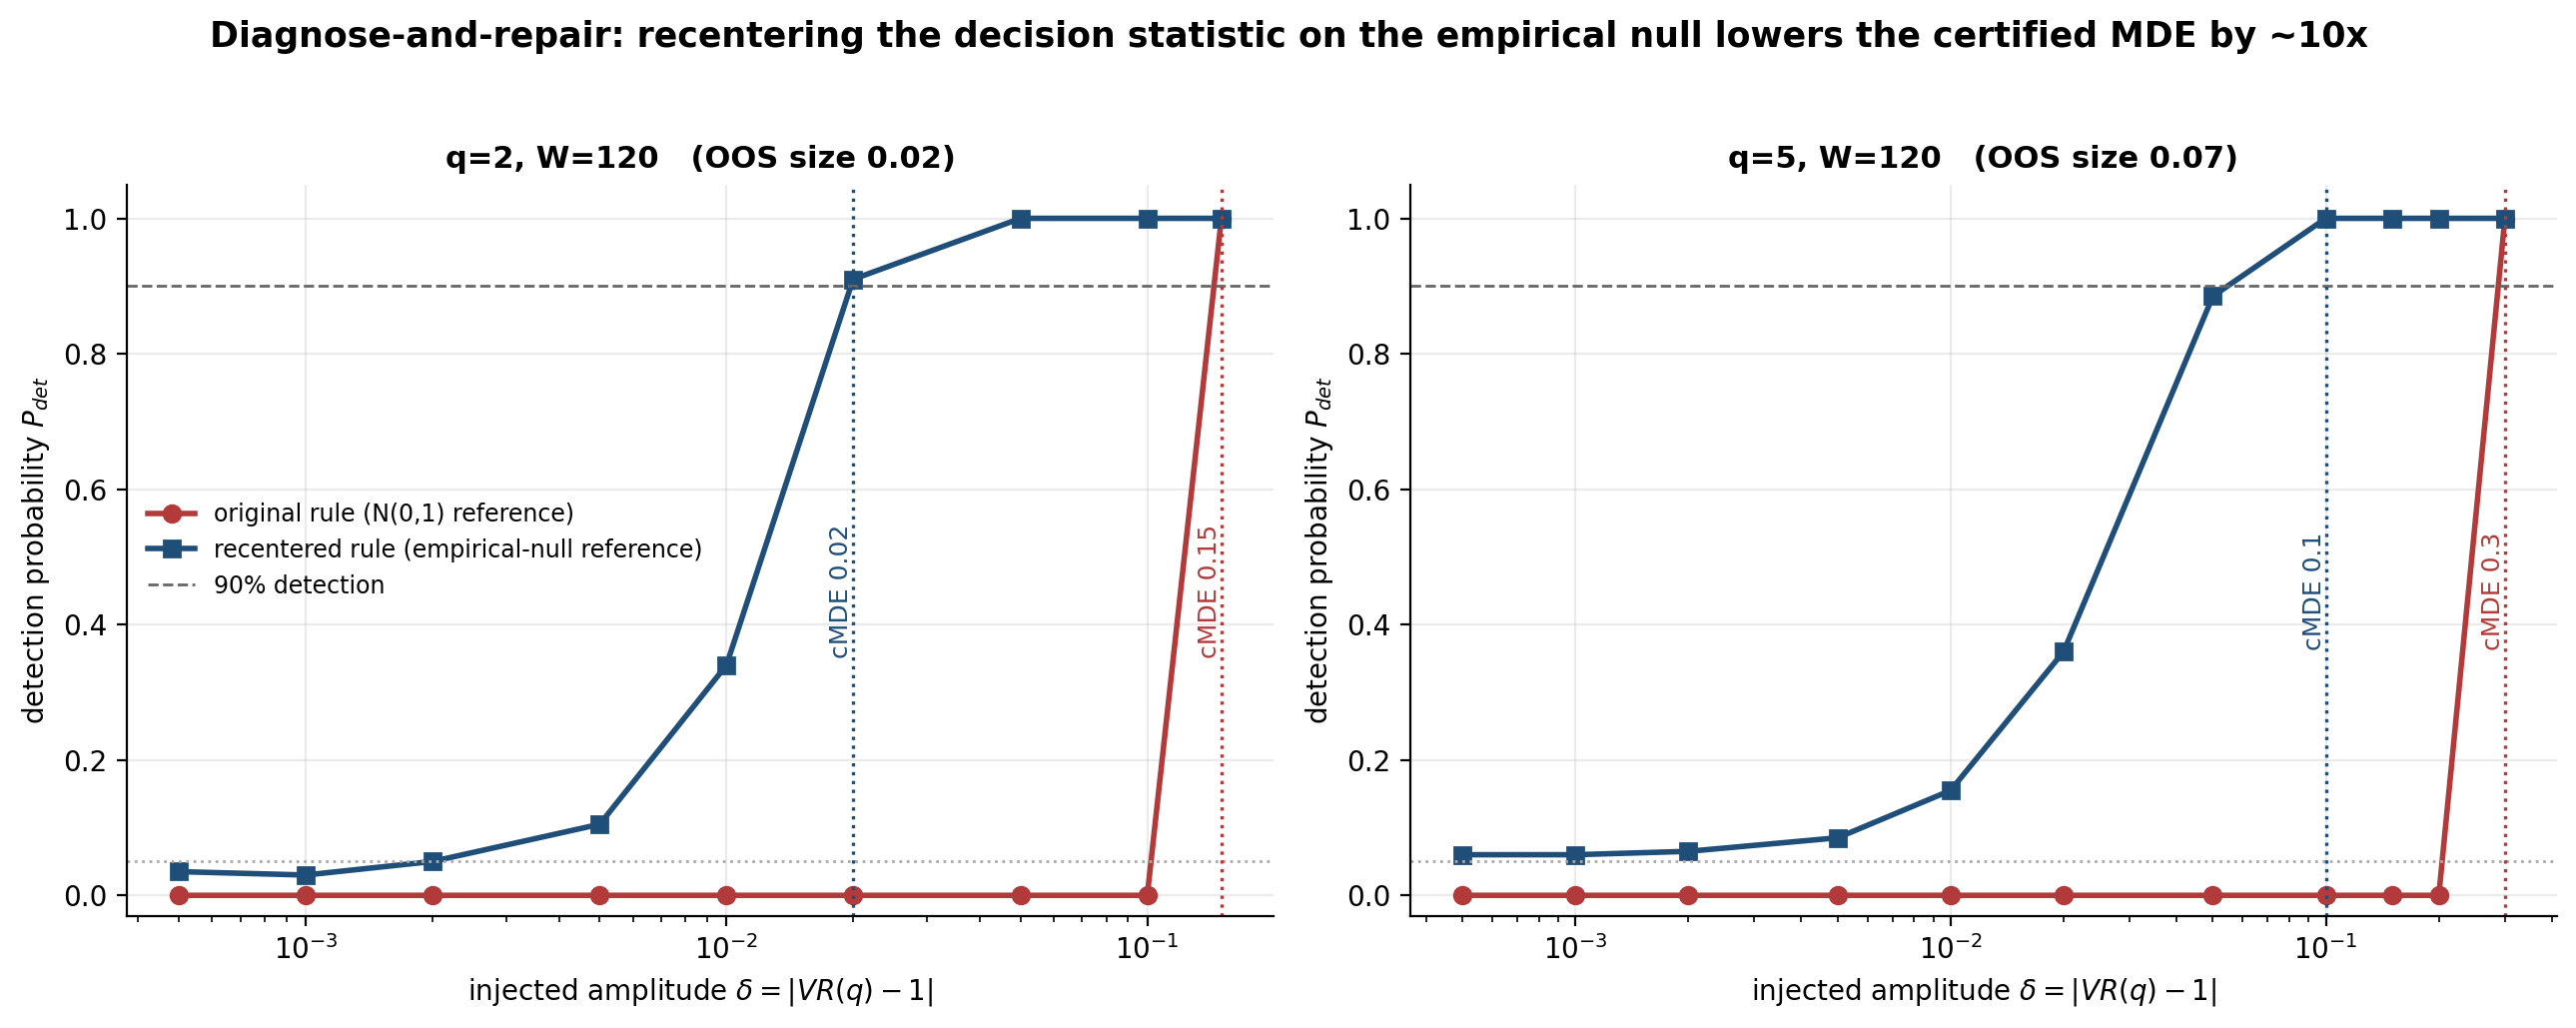
\includegraphics[width=\textwidth]{fig03_repair_power.png}
\caption{The frozen rule (red) recovers nothing below $\delta=0.15$
($q{=}2$) or $0.30$ ($q{=}5$); recentering the decision statistic on the
empirical null (blue) shifts the power curve left by roughly a decade, with
out-of-sample size held near $5\%$. The certified minimum detectable effect
falls into the preregistered amplitude grid, so the repaired instrument is
adequately powered for the declared claim.}
\label{fig:repair}
\end{figure}

Applied to the observed market, the repaired instrument does not manufacture
a detection. Recentered on its own dependence-preserving null, the observed
BTCUSDT statistic sits at $-1.9$ null standard deviations at $q{=}2$ and
$-1.8$ at $q{=}5$---on the \emph{negative} side, consistent with weak
mean-reversion, which the positive-autocorrelation gate correctly declines to
report as positive dependence. The difference from the frozen certificate is
decisive for interpretation: the withhold is no longer underpowered. With
$\mathrm{cMDE}=0.02$ at $q{=}2$, the repaired detector \emph{excludes} positive
short-horizon serial dependence above $\delta=0.02$ with demonstrated power,
converting an uninterpretable non-result into a bounded, severe negative
result in the sense of \citet{Mayo2018}.

For the scoped scientific claim---positive short-horizon ($q{=}2$) serial
dependence on calendar bars, without an economic target---the repaired
instrument now clears every applicable gate: size controlled (OOS $0.02$),
power demonstrated ($\mathrm{cMDE}=0.02$), and transport certified across all
three sampling schemes at $q{=}2$ (Table~\ref{tab:transport}). Its disposition
is therefore \textbf{admissible}---the protocol's first---and
Table~\ref{tab:cert-admissible} exhibits the completed certificate. Two
properties of this admission deserve emphasis. It was reached by repairing a
diagnosed fault, not by relaxing a gate: the recentering is the standard
empirical-null calibration the size gate itself prescribed. And admissible
does not mean the market claim is affirmed---here the admitted certificate
records a powered \emph{exclusion}, which is precisely the kind of credible
negative result that certification exists to license.

\begin{table}[htbp]
\centering
\begin{threeparttable}
\caption{First admissible certificate: recentered VR trigger, scoped claim
(positive $q{=}2$ serial dependence, calendar bars, scientific target,
BTCUSDT \dataspan).}
\label{tab:cert-admissible}
\small
\begin{tabularx}{\textwidth}{@{}lX@{}}
\toprule
Field & Certified content \\
\midrule
Claim tuple & Recentered VR trigger at $q{=}2$, $W{=}120$; target: positive short-horizon serial dependence (scientific, no economic target); calendar bars; positive AR(1) signal family; empirical-null reference from the $\delta\!=\!0.0005$ cell. Exploratory-grade (post-freeze recentering constants). \\
Size & OOS false-alarm $0.02$ $[0,0.05]$; empirical-null reference replaces the mis-centered $N(0,1)$. \emph{Pass}. \\
Power & $\mathrm{cMDE}=0.02$ ($\delta_{90}$); $\delta_{50}=0.02$; recovers the preregistered amplitude grid. \emph{Pass} for $\delta\ge0.02$. \\
Transport & Certified at $q{=}2$ for clock--volume, clock--intrinsic, and volume--intrinsic (Table~\ref{tab:transport}). \emph{Pass}. \\
Disposition & \textbf{Admissible} for the scoped claim. Empirical content: positive $q{=}2$ serial dependence above $\delta=0.02$ is \emph{excluded} on BTCUSDT with power $\ge0.9$ (observed statistic $-1.9$ SD, negative side). \\
Scope note & The economic claim remains \emph{cost-dominated} and the $q{=}5$ claim \emph{transport-uncertified} (Table~\ref{tab:cert-filled}); admission is for the $q{=}2$ scientific claim only. \\
\bottomrule
\end{tabularx}
\end{threeparttable}
\end{table}

\section{Three Detector Families Under One Protocol}
\label{sec:families}

Certification is detector-agnostic in a specific, testable sense: the same
gates, run on different detector families, must produce dispositions for
family-appropriate reasons rather than a single performance ranking. We
demonstrate this on a harmonized three-family exhibit---rolling-quantile
volatility detector, two-state Gaussian hidden-Markov filter
\citep{Hamilton1989}, and the variance-ratio cascade---run on a native-frequency
BTCUSDT block (2022-10-01 to 2022-12-31; $132{,}480$ one-minute bars;
$q$-units at native frequency; no downsampling), against a common two-state
volatility-regime target with frozen validity gates. This exhibit is
deliberately not a horse race: no agreement leaderboard is produced, and the
protocol in fact \emph{withholds} the pairwise agreement block because one
family fails validity.

\begin{table}[htbp]
\centering
\begin{threeparttable}
\caption{Three families, one protocol (BTCUSDT 2022-Q4; two-state
volatility-regime target; $89{,}222$ overlapping-valid bars; cost convention
$10$\,\bps).}
\label{tab:families}
\small
\begin{tabularx}{\textwidth}{@{}lXXX@{}}
\toprule
 & Rolling quantile & Hidden Markov & VR cascade \\
\midrule
Validity & Valid (occupancy $0.804/0.196$; per-state non-overlap counts pass) & \emph{Instrument-failed}: state 0 occupies 59 of $89{,}222$ bars ($0.07\%$); non-overlap count below frozen floor & Target gate: serial-dependence instrument, \emph{target-mismatched} for a common volatility-state headline \\
Information ($I_D$, nats) & $5.03\times10^{-4}$ [$3.47$, $6.66$]$\times10^{-4}$; perm.\ $p=0.005$ & Not interpreted (validity failed) & Not interpreted for this target \\
Net value & Gross $5.03$\,\bps\ $-$ $10$\,\bps\ $= -4.97$\,\bps: \emph{cost-dominated}. State label is always-on, so per-epoch and per-trigger conventions coincide & --- & --- \\
Missing gates & Power, size, transport not measured for this family & --- & (Certified separately in Section~\ref{sec:empirical}) \\
Disposition & \emph{Cost-dominated} (gate 6 fails on measured evidence, so the missing-estimand fallback does not apply; incomplete power/size/transport coverage recorded in the profile) & \emph{Instrument-failed} (gate 1: read before any statistical gate) & \emph{Target-mismatched} (gate 2) for this claim \\
\bottomrule
\end{tabularx}
\begin{tablenotes}\footnotesize
\item Pairwise agreement metrics (Cohen's $\kappa$, adjusted Rand, NMI) were
withheld by the protocol---the artifact's pairwise block is empty---because a
family member failed validity gates; run-level disposition:
\texttt{instrument\_failure}. The three-state variant of the task yields the
same dispositions (rolling-quantile $I_D=5.47\times10^{-4}$ nats,
$p=0.005$).
\end{tablenotes}
\end{threeparttable}
\end{table}

Three families, three dispositions, three different reasons---none of them a
relative performance statement. The hidden-Markov failure is the precedence
rule working as designed: a degenerate fit (one state absorbing $99.9\%$ of
bars) is an instrument failure to be reported \emph{before} any information
or agreement number is interpreted---and it is a repairable fit (constrained
re-estimation or a longer window would likely populate both states), not a
data point about hidden-Markov models in general. The rolling-quantile
detector shows the intermediate state the rule produces when evidence is
partial: its measured value gate fails ($W_D=-4.97$\,\bps), so the
disposition is \emph{cost-dominated} on measured evidence, while the
unmeasured power, size, and transport gates are recorded as missing coverage
rather than silently extrapolated. The cascade's exclusion from a
volatility-state headline is target eligibility, not failure. A leaderboard
over these three streams would have converted an instrument failure, a
target mismatch, and a cost-dominated value gate into a performance ranking;
the protocol instead reports each for what it is.

\section{What Certification Changes in Practice}
\label{sec:discussion}

Certification and the comparison toolkit answer different questions and
compose in order. A reality-check, SPA test, or model confidence set
\citep{White2000,Hansen2005,HansenLundeNason2011} asks which candidate beats
a benchmark, presupposing each label stream is a valid measurement of a
common object; the certificate asks the prior question of whether that
presupposition holds, and reports what no relative test does---mis-centered
size, failed transport, convention-dependent value. Certification comes
first (which outputs may enter), comparison second (among admitted outputs
only).

\paragraph{For the empirical researcher}, the certificate converts negative
results into bounded evidence with a stated power pedigree---the format that
post-replication-crisis empirical finance explicitly calls for
\citep{Harvey2017,HouXueZhang2020}. A regime paper whose detector is
certified underpowered below $\delta=0.15$ cannot claim the market has no
regimes; it can claim, defensibly, that departures above the threshold are
excluded.

\paragraph{For the model validator}, the certificate is a model-risk artifact
in the sense of \citet{FederalReserveOCC2011}: a pre-use validation with
explicit expiry and recalibration triggers, extending VaR-style backtesting
\citep{Kupiec1995,Christoffersen1998} to label-producing models that current
backtesting practice does not cover.

\paragraph{For the trading researcher}, the value gate separates three
routinely conflated objects: information in the market path (a ceiling, by
Corollary~\ref{cor:dpi}), information in the detector output (the estimand),
and value net of a declared cost convention (the gate). The demonstrated
convention-dependence is a caution against both optimistic and pessimistic
shortcuts: charging every epoch a full round-trip buried a positive
per-trigger bound; per-trigger accounting, taken alone, would overstate what
an upper bound licenses. The certificate's answer is not a number but a
frozen convention plus a disclosed sensitivity.

\section{Domain of Validity, Limitations, and Sequential Extension}
\label{sec:validity}

Every empirical statement in this paper is bounded by
Table~\ref{tab:validity}, and we make the boundaries explicit rather than
relying on generalization by analogy. Three limitations deserve emphasis.
First, the size diagnostic runs at $B=100$: it demonstrates the gate and
bounds the false-alarm rate below $3.6\%$, but a deployment certificate
requires a pre-declared budget sized to its resolution target, across
multiple null families. Second, power, size, and transport were measured for
one detector family; the three-family exhibit shows the protocol's refusal
states on other families, not their full certificates---completing a non-VR
certificate is the natural next study, and the \emph{incomplete} disposition
is the protocol saying so itself. Third, the injection design perturbs the
empirical path with a single signal family (positive AR(1) calibrated to
$|\VR(q)-1|$); a claim about a different signal shape requires refreezing
$s$. A specification-curve presentation of the certificate across reasonable
tuple variations \citep{Simonsohn2020}---and multi-asset extensions run as
registered reports---are the two designed-in growth paths for the evidence
base.

\begin{table}[htbp]
\centering
\caption{Domain of validity of the empirical claims.}
\label{tab:validity}
\small
\begin{tabularx}{\textwidth}{@{}lX@{}}
\toprule
Dimension & Certified scope \\
\midrule
Detector & Frozen Holm-corrected LM variance-ratio cascade with positive median gate (Section~\ref{sec:empirical}); rolling-quantile and HMM families touched only by the gates shown in Table~\ref{tab:families}. \\
Asset/venue & BTCUSDT Binance USD-M perpetual futures; ETHUSDT same-venue replication in \ref{app:eth}; EUR/USD used for cost-term instantiation only (\ref{app:eurusd}). \\
Period & Development \dataspan\ (2021-05-29 to 2025-12-31); disjoint 2026-01-01 to 2026-05-29 evaluation block. \\
Frequency/schemes & One-minute base bars; calendar, volume, event-time constructions per the frozen calibration table. \\
Horizons & $q\in\{2,5,15,60\}$ bars; windows $W\in\{60,120,240\}$. \\
Signal family & Positive AR(1) injections targeting $|\VR(q)-1|\in[0.0005,0.30]$ as executed. \\
Nulls & Centered circular block bootstrap, block 120, $B=100$ (resolution-limited as stated). \\
Costs & $10$\,\bps\ all-in round-trip at unit size; per-epoch attribution frozen, per-trigger sensitivity disclosed; EUR/USD spread evidence for cost-term instantiation. \\
Claims excluded & Any profitability claim; any market-efficiency verdict; any cross-asset or cross-family generalization beyond the rows above. \\
\bottomrule
\end{tabularx}
\end{table}

\paragraph{Sequential extension.} Production use needs a monitoring form of
the protocol: admit a detector when rolling evidence first clears the gates,
revoke when it degrades. A window-by-window p-value monitor is the wrong
instrument---continuous looking with optional stopping invalidates its
nominal guarantees, a problem known since sequential monitoring of structural
change \citep{ChuStinchcombeWhite1996}. Proposition~\ref{prop:online-e}
supplies the correct instrument: monitoring each gate by an e-process makes
admission anytime-valid, so the false-admission probability is bounded over
an unbounded horizon under optional stopping, with no error budget split
across gates or looks. This is a stronger and simpler guarantee than the
fixed max-statistic budget of the earlier prototype. The remaining step is
empirical: the repository's prototype state machine replays a \emph{scripted}
schedule rather than calibrated e-processes, which under this paper's own
rules is not admissible evidence, so we report the guarantee and its
construction but withhold a sequential empirical demonstration until the
monitor is rebuilt on the betting e-process of Section~\ref{sec:evalue} and
certified against replayed history.

\section{Conclusion}
\label{sec:conclusion}

Regime detectors are measurement instruments, and this paper's proposal is
that they be treated with an instrument's discipline: no output enters
inference or allocation until its power, false-alarm behavior,
transportability, and net information value have been measured for one
frozen claim. The deliverable is the certificate, and a withheld admission
carries as much usable information as a granted one, because it names the
failed gate.

The demonstration certifies a variance-ratio cascade on five years of
one-minute Bitcoin futures and withholds admission, for measured reasons:
the rule's empirical false-alarm rate sits significantly below its nominal
level, with a mis-centered asymptotic reference---a size distortion in the
conservative direction; a preregistered 96-cell grid shows the cascade
cannot detect departures at any amplitude up to $0.10$, with the response
threshold bracketed at $(0.10,0.15]$ at $q{=}2$ and $(0.20,0.30]$ at
$q{=}5$; labels transport across calendar, volume, and event-time bars at
$q{=}2$ but not at the primary horizon; and trigger information, resolvable
at $q{=}5$, has a net value whose sign depends on a cost-attribution
convention that the certificate therefore freezes and discloses. A
three-family exhibit shows the same protocol returning instrument-failed,
target-mismatched, and cost-dominated dispositions rather than a
leaderboard.

None of this is a verdict on Bitcoin's efficiency, on variance-ratio tests,
or on any trading strategy. It is a worked template for a validation step
that regime-detection practice currently skips: bounded claims, measured
power, disclosed provenance, and refusal as a reportable outcome.

\appendix

\section{Derivations}
\label{app:derivations}

\paragraph{Proposition~\ref{prop:power}.} Conditional on the empirical path
$X$, the injection design, and the frozen rule, each Monte Carlo draw applies
independent injection randomness to the same measurable event
$\{D_\theta(T_g(J_{\delta,s}(X)))\ \text{fires}\}$; draw outcomes are
i.i.d.\ Bernoulli$(\Pdet)$ by construction of the simulator, so the sample
fire rate is the maximum-likelihood estimator of $\Pdet$ and Clopper--Pearson
intervals are exact at any $N_{\mathrm{mc}}$. The conditionality is
irreducible: nothing licenses extrapolation beyond the declared path, family,
and grid.

\paragraph{Proposition~\ref{prop:transport}.} Immediate from the definition
of certification: a transported claim requires certified equivalence of the
declared statistics; absent certification, the transported claim has no
measured basis, which is the withholding rule. The content is operational,
not probabilistic.

\paragraph{Proposition~\ref{prop:cost} and Corollary~\ref{cor:dpi}.} The
fair-odds log-optimal bound gives expected log-growth advantage at most
$I(D;Y)$ nats per decision \citep{Kelly1956,AlgoetCover1988,CoverThomas2006};
converting to basis points and subtracting the declared cost under the
declared attribution convention yields $W_D$; non-positive $W_D$ excludes
detector-only use under that convention, and positivity remains an upper
bound because the Kelly bettor is idealized (perfect odds, no constraint, no
estimation error). The corollary is the data-processing inequality applied to
the causal map $X_{\le t}^g \mapsto D_t^g$.

\paragraph{Proposition~\ref{prop:static-e}.} Under $H_0=\bigcup_k H_0^k$ there
is a gate $k^\ast$ with $H_0^{k^\ast}$ true. Admission requires
$E_{k^\ast}\ge1/\alpha$, so by Markov's inequality and the e-value property,
$\Pr_{H_0}(\text{admit})\le\Pr_{H_0^{k^\ast}}(E_{k^\ast}\ge1/\alpha)
\le\alpha\,\mathbb{E}_{H_0^{k^\ast}}[E_{k^\ast}]\le\alpha$. No union over
gates appears because admission is a conjunction; the bound is controlled by
the single true null. That the product of fold-wise e-values and the average
of arbitrary e-values are themselves e-values are, respectively, the tower
property and linearity of expectation \citep{VovkWang2021}.

\paragraph{Proposition~\ref{prop:online-e}.} Under $H_0$ some gate $k^\ast$
fails at all $t$, so $(E^{k^\ast}_t)$ is a nonnegative supermartingale with
$\mathbb{E}[E^{k^\ast}_0]\le1$. Ville's inequality gives
$\Pr(\exists\,t:E^{k^\ast}_t\ge1/\alpha)\le\alpha\,\mathbb{E}[E^{k^\ast}_0]
\le\alpha$. Admission at any $t$ requires $E^{k^\ast}_t\ge1/\alpha$, hence
$\Pr(\exists\,t:\text{admit})\le\alpha$; the bound is uniform over $t$ and so
survives any data-dependent stopping rule \citep{Ramdas2023}.

\section{ETHUSDT External Replication}
\label{app:eth}

The full workflow was rerun on ETHUSDT Binance USD-M perpetual futures at
one-minute frequency, same effective window as BTCUSDT (2021-05-29 to
2025-12-31, $n=\numbars$ bars) and same disjoint 2026 block (through
2026-05-29, $n=214{,}355$ bars). The run changes the asset symbol only; BTC
injection artifacts are not reused as ETH calibration data, and no
ETH-specific injection grid or empirical-size run exists
(\texttt{eth\_specific\_injection\_grid: false}), so the ETH certificate is
\emph{incomplete} by its own provenance---exactly the disposition the
protocol requires rather than a silent extrapolation.

Measured gates replicate the qualitative BTC pattern with instructive
differences. Primary cell: median $|\VR(5)-1|=0.1609$ (mean $0.1832$),
median standardized statistic $-0.3981$, asymptotic p $=0.691$, cascade
silent---large departure, wrong sign for the positive gate, below the
demonstrated response threshold. Transport (same margin, same 12-row family):
certified at $q{=}2$ for clock--volume ($\widehat{\Delta}=0.0035$, Holm
$6.2\times10^{-42}$) and volume--intrinsic ($0.0094$, Holm $0.014$) but
\emph{not} clock--intrinsic ($0.0129$, Holm $0.154$); certified at $q{=}5$
for clock--volume ($0.0110$, Holm $0.0014$) and at $q{=}60$ for
clock--volume ($0.0050$, Holm $0.0043$); all event-time pairs at $q\ge5$
fail, with the $q\ge15$ rows precision-limited as on BTC. The certified set
differs from BTCUSDT's---transport certification is an asset-specific
measurement, not a detector constant, which is the point of gating it.
Persistence diagnostics reject the dependence-preserving null
(KS $=0.261$, bootstrap p $<0.001$), and the disjoint 2026 block repeats the
primary-cell disposition ($|\VR(5)-1|=0.1568$, median $Z=-0.3126$,
p $=0.755$, $1{,}786$ windows). Raw sign-pair information bounds
($9.2$\,\bps\ gross at $q{=}5$) are recorded in the artifact as scale
diagnostics only and are not detector evidence under
Corollary~\ref{cor:dpi}.

\section{EUR/USD Cost-Term Instantiation}
\label{app:eurusd}

Daily reference FX rates contain no executable quotes, so using them for the
cost gate would force a frictionless exception to Equation~\eqref{eq:wd}. The
repository instead instantiates the cost term from free HistData Generic
ASCII tick quotes with bid, ask, and volume: 56 monthly files,
$113{,}650{,}998$ EURUSD ticks, aggregated to $1{,}659{,}616$ one-minute
last-quote bid/ask bars over a BTC/ETH-matched window (2021-05-29 19:32 UTC
to 2025-12-31 23:59 UTC; first available quote 2021-05-30 17:00, last
2025-12-31 16:58, reflecting FX session hours). Median observed spread:
$3.0\times10^{-5}$ ($0.284$\,\bps\ of mid); mean $0.417$\,\bps; matched-span
maximum $30.95$\,\bps. This appendix is deliberately narrow: it shows the
certificate's cost term can be instantiated on a traditional asset without
paid institutional data, and it is not a second-asset detector certificate
(power, size, transport, and information gates were not run under an FX
claim tuple).

\section{Reproducibility and Legacy Naming}
\label{app:repro}

The replication package separates method, claim boundaries, code, tests, and
frozen evidence. Three reproduction levels are supported: (i) rebuild the
manuscript and check every reported value against the frozen artifacts via
the claim-traceability ledger; (ii) run the focused verification tests
against the included scripts and artifacts; (iii) regenerate comparable
artifacts from independently obtained raw data using the documented commands.
Raw venue and vendor data are not redistributed.

The package separates the manuscript and figures (\path{paper/}), the claim
boundary (\path{CLAIMS.md}, \path{CLAIM_TRACEABILITY.md},
\path{ARTIFACT_LEDGER.md}), the method implementation (\path{scripts/wp1/},
\path{src/strategies/vol_regime_switch/}), the frozen evidence
(\path{data/injection_runs/}, 104 power cells; \path{backtest_results/} for
the size, transport, information, disjoint-window, replication, benchmark,
reference-repair, and cost artifacts), and the verification tests
(\path{tests/wp1/}); raw Binance USD-M and HistData inputs are identified in
the runbook but not redistributed.

Integrity conventions: the detector and claim tuple are frozen before
interpretation (preregistration commits recorded in every artifact); the 2026
block is excluded from development by a recorded loader flag; seeds and
bootstrap settings are stored in scripts or artifacts; derived artifacts are
immutable evidence anchors; post-freeze evidence carries an explicit
exploratory flag that the manuscript must disclose wherever such evidence is
displayed; and regeneration writes new output paths unless manuscript and
ledger are updated together.

\emph{Legacy naming.} The protocol was developed in the repository under the
working name GCDE (``gauge-calibrated detector exclusion''), and frozen
artifact paths and keys retain that vocabulary (\path{gauge_invariance/},
\texttt{gauge\_scope}, \path{thermodynamic_bound/}). The correspondence is:
gauge $\to$ sampling scheme / market clock; gauge defect $\to$ transport
discrepancy $\Delta_D$; available decision work $\to$ net information value
$W_D$; exclusion $\to$ withheld admission; failure fingerprint $\to$ failure
profile. Artifact keys are quoted verbatim where they appear so that ledger
lookups remain exact.

\section*{Data and Code Availability}

The demonstration uses locally archived Binance USD-M BTCUSDT and ETHUSDT
one-minute perpetual futures data, a free matched-span HistData EURUSD
bid/ask sample, and frozen derived artifacts in the project repository.
Principal scripts: \path{scripts/wp1/}; verification tests:
\path{tests/wp1/}; frozen artifacts: \path{data/injection_runs/} and
\path{backtest_results/}; evidence map: the artifact ledger and claim
traceability files. The public replication repository mirrors the paper
package structure. Raw market-data redistribution is subject to the original
venue and vendor terms.

\bibliography{references}

\end{document}
